\chapter{The Geometry of Conceptualisation: Analogies} \label{chap:analogy}
In this chapter, as a final empirical investigation into the potentialities of context specific distributional semantic techniques, I will investigate the capacity of my methodologies to model analogy.  For the purposes of the computational and geometric modelling of semantics, analogy can be seen as a kind of meta-phenomenon: an analogical equation involving two sets of lexical representations indicates that there is some underlying intensionality that conceptually binds the denotations of the representations.  So, for instance, the metaphor ``that surgeon is a butcher'' can be extended through a mapping between the conceptual domains of \textsc{surgery} and \textsc{butchery} to arrive at semantic formulae such as \emph{surgeon:scalpel :: butcher:cleaver} or \emph{hospital:patient :: abattoir:carcass}.  Furthermore, if these relationships can be mapped geometrically in a semantic space, then we should have on our hands a productive mechanism for configuring a general semantic model---and one which may overcome some of the issues of interpretation and composition raised in the last chapter.  If we can connect a general region of butchery to a region of surgery in a semantic space, for instance, then we might be able to extrapolate such metaphoric turns of speech as ``the surgeon hacked at me with her scalpel'' from a model without committing to the claim that the model (or, for that matter, an agent) has actually interpreted the metaphor in an online way.

The idea that there is a geometric component to analogy is at least hinted at by \cite{Tversky1977}, who, as discussed in Chapter~\ref{sec:frames}, raises the issue of inequalities and asymmetries in relationships of synonymy.  \cite{Gentner1983} extends Tversky's insights to a model explicitly targeting analogy through the application of isomorphic \emph{structure mappings} that identify congruities between conceptual domains based on composite symbolic representations.  From a computational perspective, \cite{VealeEA1992} describe a system that functions through a series of \emph{spatial operators} which facilitate mappings between conceptual domains by way of a schema of collocations, containments, and orientations, though these operations do not involve the instantiation of Euclidean measures.  Subsequent symbolic computational models of metaphor in particular have seized on the mechanism of modelling mappings between conceptual structures that are, to a greater or lesser extent, based on the identification of congruities and a corresponding geometrical logic of sorts, and a small sample of work in the field has been surveyed in Chapter~\ref{sec:words} and \ref{sec:metaback}.

The empirical work described here will, naturally, focus on a statistical rather than symbolic approach to modelling analogy by way of spatial mappings between domains---and, in this case, domains, in the spirit of \cite{Gardenfors2000}, are represented roughly as regions in a Euclidean space.  It is important to note, though, that one of the primary components of the productive symbolic approaches to analogy mentioned above goes away once we move into distributional semantic spaces: where the features of symbolic representations are generally constructed to be interpreted as actual attributes of the denotations being modelled, the dimensions of distributional semantic spaces are simply indices to information about co-occurrences observed in a digital corpus (this has already been discussed in Chapter~\ref{sec:litdims} in the context of \citepos{Rimell2014} work studying the relationship between co-occurrence overlap and entailment, and again in Chapter~\ref{sec:interpretable} by way of \citepos{DerracEA2015} model treating directions in factorised distributional spaces as conceptual themes).  So there is a trade-off between access to a continuous Euclidean space of lexical semantic representations with geometric measures facilitated by the statistical nature of the representation building process and the loss of interpretable features in a symbolic conceptual scheme.  My hypothesis here, in line with experiments described in the previous two chapters, is that a process of contextualisation can generate spaces where collections of co-occurrence dimensions representing conceptually oriented profiles of language use will provide an appropriate ground for modelling analogy in terms of rigorous Euclidean relationships.  And in the case of analogy in particular, as will be seen in the following section, there is already a body of work offering compelling evidence that distributional semantic statistics can map conceptual relationships onto the geometry of word co-occurrence.

\section{Analogies as Parallel Vectors} \label{sec:parallel}
The \texttt{word2vec} distributional semantic modelling techniques, which have served as a point of comparison and discussion throughout this thesis, were originally presented with a test set of 19,544 four-word analogies, constructed by the model artchitects and devised to cover a range of relationships which the designers categorised as broadly \emph{semantic} or \emph{syntactic} \citep{MikolovEA2013b,MikolovEA2013c}.\footnote{The analogy data is included in the package that can be downloaded at \url{https://code.google.com/archive/p/word2vec/source/default/source}.}  So, for instance, the data presents relationships such as, on the one hand, \emph{Bangkok:Thailand :: Paris:France} or \emph{boy:girl :: man:woman}, and, on the other hand, \emph{calm:calmly :: lucky:luckily} or \emph{aware:unaware :: efficient:inefficient}.  The task involves feeding a semantic model the first three terms and then measuring the rate at which it is able to accurately predict the fourth term.

The neural network architecture of the \texttt{word2vec} approach produces remarkably strong results on this task through the application of a simple geometric device.  Within the normalised space of word-vectors generated over the course of iterative traversals of a large-scale digital corpus, given an unfinished analogy of form \emph{A:B::C:X}, the model simply finds the vector $\overrightarrow{x}$ most closely fulfilling the equation $\overrightarrow{b} + \overrightarrow{c} - \overrightarrow{a} \approx \overrightarrow{x}$, where $\overrightarrow{a}$, $\overrightarrow{b}$, and $\overrightarrow{c}$ are the word-vectors corresponding to the three known elements of the analogy, and returns the vocabulary word associated with $\overrightarrow{x}$.  The original literature reports an accuracy rate of 0.61 for the CBoW model, which is all the more impressive when we consider how many ways there are to choose the wrong solution to an analogy from a vocabulary of one million words.  \citep[It should be noted that similarly strong results have been reported for the hybrid frequentist-neural model of][.]{PenningtonEA2014}

But the really remarkable thing about these results is that the models build these spaces in a completely unsupervised manner with respect to the actual task of analogy solution.  This means that the arrangement of word-vectors plays out in a tidy conceptual geometry, interpretable through simple linear algebraic operations, simply by virtue of the way that words tend to come up in proximity to one another in the course of colloquial written language use (the original results were obtained from models trained on the Google News Corpus, and, as will be seen below, the same models trained on Wikipedia achieve comparable scores).  Much has been made of this: \cite{LevyEA2014} postulate about the procedural equivalence of iterative and statistical models mitigated by parameterisation issues, while \cite{AroraEA2015} have attempted to explain mathematically how the application of a random walk type algorithm to statistical models results in a recapitulation of the strong neural network results.  At the time of writing, there is a generally accepted intuition afoot in the field that, along the lines of the distributional hypothesis itself, it makes sense that the gradual nudging of word-vectors by a neural network based on observations of co-occurrences should push words into situations where orientations and distances in space broadly map to conceptual relationships between representations; there is not, however, a well-formed mathematical explanation of why these techniques are so effective at projecting semantic relationships into space.  At any rate, the import of all this is that, in \texttt{word2vec} type distributional semantic spaces, at least a certain type of analogy plays out along the lines illustrated in Figure~\ref{fig:sense}, as a close approximation of a parallelogram at the surface of a normalised hypersphere in a space delineated by abstract dimensions acting as handles for the backpropagating action of a neural network.

\begin{figure}
%  \centering
  \begin{subfigure} [t] {0.5\textwidth}
  \centering
  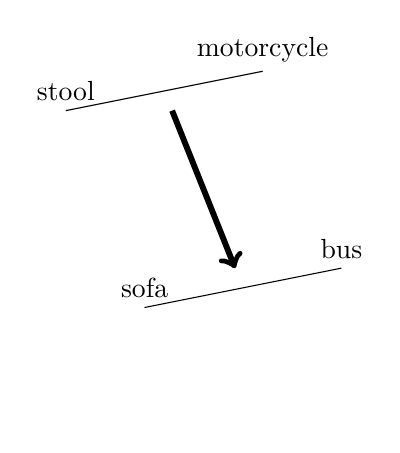
\begin{tikzpicture} [scale = 0.05]
    \draw (10,80)--(60,90);
    \draw (10,80) [above] node {stool};
    \draw (60,90) [above] node{motorcycle};
    \draw (30,30)--(80,40);
    \draw (30,30) [above] node {sofa};
    \draw (80,40) [above] node {bus};
    \draw [->,line width = 0.75 mm] (37,80)--(53,40);
    \draw (60,10) [below,white] node {soft};
  \end{tikzpicture}
  \caption{This makes sense.}
  \label{fig:sense}
  \end{subfigure}
  \begin{subfigure} [t] {0.5\textwidth}
  \centering
  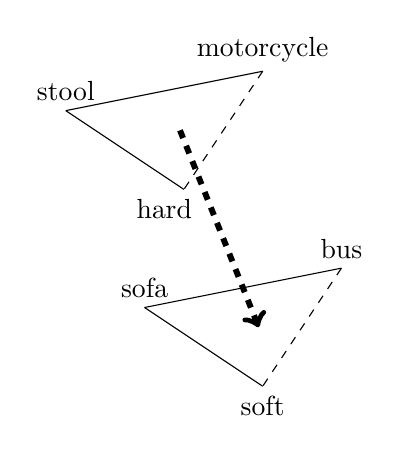
\begin{tikzpicture} [scale = 0.05]
    \draw (10,80)--(60,90);
    \draw (10,80)--(40,60);
    \draw [dashed] (60,90)--(40,60);
    \draw (10,80) [above] node {stool};
    \draw (60,90) [above] node {motorcycle};
    \draw (35,60) [below] node {hard};
    \draw [->,line width = 0.75 mm,dashed] (39,75)--(59,25);
    \draw (30,30)--(80,40);
    \draw (30,30)--(60,10);
    \draw [dashed] (80,40)--(60,10);
    \draw (30,30) [above] node {sofa};
    \draw (80,40) [above] node {bus};
    \draw (60,10) [below] node {soft};
  \end{tikzpicture}
  \caption{Does this make sense?}
  \label{fig:nonsense}
  \end{subfigure}
\caption[Analogies Straining Geometry]{The analogical components of overlapping conceptual frames do not necessarily map neatly into a singular space.}
\label{fig:mismatch}
\end{figure}

So, to put it in plain language, the line between two points representing a conceptual relationship in one region of the space should be parallel to and in the same direction as two points in another region representing an analogous conceptual relationship under a different overall conceptual scheme.  There is, however, an objection to be raised here.  Returning once again to \citepos{Tversky1977} observations about the asymmetry of similarity, there are problems once we begin to extend the geometry of analogy to more complex conceptual structures, as illustrated in Figure~\ref{fig:nonsense}: for any given mapping between anything other than the most trivial conceptual domains, there will be some intensional component of the denotation that does not conform to the presumed isomorphism of the analogy in a distributional semantic space.  So, while it may be possible to map relatively atomic elements analogically in a space of fixed semantic points, it seems there will always be a breakdown when it comes to trying to discover isomorphisms between entire domains.

As will be recalled from Chapter~\ref{sec:frames} and the example involving moethers, nurses, and frogs, \cite{ChenEA2017} have noted geometrical anomalies specifically in the context of distributional semantics, demonstrating that the presumption of conceptual parallelism is considerably more consistent in some domains than others, and further using clinical studies on human respondents to feel out some of the disconnects in analogical chains inherent in these types of semantic models.  What becomes clear is that static distributional models are very effective at providing a semantically productive geometry some of the time, but they lack the adaptability that is fundamental to environmentally situated cognition and so do not make the open-ended kind of connections between words and concepts that are characteristic of semantics.  What is necessary is an element of flexibility, and I propose that my methodology for contextualising semantic spaces offers the proper kind of framework for providing the required sensitivity to unfolding situations in the world.

\section{Contextualising Analogical Geometry} \label{sec:anatext}
In this section, I will explore the distributional contexts of analogical semantic relationships.  The premise of this investigation arises from the disconnect illustrated in Figure~\ref{fig:mismatch}: it seems impossible to imagine how a static semantic space could consistently represent analogies as well-formed geometric entities.  Rather, I maintain that analogy is always to at least a certain extent context specific.  Following on this, my hypothesis is that there should almost always be some contextualisation which permits the satisfactory mapping of an analogy in a semantic space.  In the case of a simple four word lexical construct, which will be the focus of the work presented here, this means that an analogy is modelled as a parallelogram, with each of the word-vectors denoting the components of the analogy as a vertex, to a degree of precision that precludes any other word-vector from being mistaken as a component of the lexical-conceptual complex.

The empirical work described here will proceed initially with a strategy of reverse engineering of sorts, seeking to validate the possibility of discovering the kind of spaces that we would like to find for mapping analogies through contextualising operations on distributional semantic spaces delineated by literal co-occurrence dimensions.  This will lead on to an examination of some of the ways that context sensitive approaches might be applied to an analogy completion task, though, not surprisingly, it turns out to be considerably easier to find a space where an analogy works out as desired than to discover an analogy in the sizeable state space of possible subspaces.  In the end, this last empirical component to my research, which expands upon work originally presented in \cite{McGregorEA2016}, will hopefully serve as an incipient to further research in terms of the potentialities and capacities of context sensitive distributional semantics.

\subsection{Projecting Probability into Space} \label{sec:anamath}
Before we engage with an exploration of the analogical potential of context specific subspaces, a brief review of the mathematics of distributional semantic spaces with literal co-occurrence dimensions will serve to reinforce the connection between the geometry of analogy and the probabilistic grounding of my methodology.  Returning to the definition of a co-occurrence statistic outlined in Chapter~\ref{sec:math}, recall that the pointwise mutual information between a word $w$ and a co-occurrence term $c$ is the unexpectedness associated with an observation of $c$ in proximity to $w$, which can be expressed in terms of joint and compound probabilities (and the equation is approximate because we're ignoring the skewing factor of 1 and the smoothing constant described in Chapter~\ref{sec:pmi}):

\begin{equation}
PMI(w,c) \approx \log\left(\frac{p(w,c)}{p(w) \times p(c)}\right)
\end{equation}

\noindent The basic assumption of the geometric approach to analogy, meanwhile, is that the components of an analogy map into a parallelogram sitting in some askance situation in a high dimensional space, a state of affairs which can be expressed using linear algebraic terms for a suppositional analogy \emph{A:B::C:D} and the corresponding word-vectors:

\begin{equation}
\overrightarrow{a} - \overrightarrow{b} \approx \overrightarrow{c} - \overrightarrow{d}
\end{equation}

\noindent For any arbitrary dimension $i$, this can then be reduced to a difference between logs:

\begin{equation}
\log\left(\frac{p(a,i)}{p(a) \times p(i)}\right) - \log\left(\frac{p(b,i)}{p(b) \times p(i)}\right) \approx \log\left(\frac{p(c,i)}{p(c) \times p(i)}\right) - \log\left(\frac{p(d,i)}{d(a) \times p(i)}\right)
\end{equation}

\noindent This expression can be significantly reduced by merging the arguments of the logarithms on either side of the equation into ratios and then dropping the logs:

\begin{equation}
\frac{p(a,i) \times p(b)}{p(b,i) \times p(a)} \approx \frac{p(c,i) \times p(d)}{p(d,i) \times p(c)}
\end{equation}

\noindent Or, converting the ratio of joint and independent probabilities to conditional probabilities and with a little more algebra:

\begin{equation}
p(i|a,i|d) \approx p(i|b,i|c)
\end{equation}

\noindent To again state this plainly, our analogy optimisation function seeks to find those dimensions where the combined probability of observing a given co-occurrence term in the context of $A$ and also (though not necessarily simultaneously) $D$ is as close as possible to observing the same term in the contexts of $B$ and $C$.  So for instance we are interested in discovering a dimension that is about as likely to occur in a context of \emph{surgeon} and \emph{cleaver} as it is to occur in a context of \emph{butcher} and \emph{scalpel}.  If we can discover a profile of such dimensions, then we can productively map this particular analogy onto a contextualised distributional semantic space.

This property of semantic spaces defined in information theoretical terms is an artefact of the conversion of products and ratios into sums and differences through the mechanism of logarithmic functions.  To coin a term, logarithms \emph{geometrise} a space of probabilistic statistics, allowing us to perform operations on shapes in Euclidean space that correspond to hypotheses about joint and conditional observations of events, in this case co-occurrence events in a large scale corpus.  It must be emphasised, however, that the interpretability of probabilities in geometric terms only holds in spaces where dimensions still map to literal co-occurrence statistics, and so this property is a feature of my methodology but not of semantic spaces that have been factorised or learned through the abstract operations of a neural network.  The next objective, then, is to search for the appropriate techniques for specifying a context in order to map out a given analogy.

\subsection{Finding Contexts for Analogies}
I next investigate whether or not co-occurrence dimensions satisfying the conditions laid out above can be discovered in co-occurrence subspaces contextualised using the methods developed and explored throughout this thesis.  In particular we are interested in discovering the dimensions which most closely satisfy the equation $(\overrightarrow{a} - \overrightarrow{b}) - (\overrightarrow{c} - \overrightarrow{d}) = 0$ for the word-vectors corresponding to the components of the analogy \emph{A:B::C:D}.  This relationship can be examined on a dimenion-by-dimension basis, beginning by extracting dimensions that are known to have non-zero values for some or all of the word-vectors involved in the analogy.  Figure~\ref{fig:histograms} presents a histographic analysis of just such an analysis for two different analogies: the aforementioned \emph{surgeon:scalpel :: butcher:cleaver}, representing the frequently discussed conceptual mapping from \textsc{surgery} to \textsc{butchery}, and, from Figure~\ref{fig:mismatch}, \emph{stool:sofa :: motorcycle:bus}, indicating a mapping from \textsc{furniture} to \textsc{vehicles}.  In both cases the best three dimensions for satisfying the balance of values indicating parallel relationships between the legs of the analogy are selected from the top 400 dimensions projected from 5x5 word co-occurrence window based spaces taking the first three of the four components of each analogy as input to the \textsc{zipped} methodology.

\begin{figure}
\begin{subfigure} {1 \textwidth}
\centering
\begin{subfigure} [t] {0.3 \textwidth}
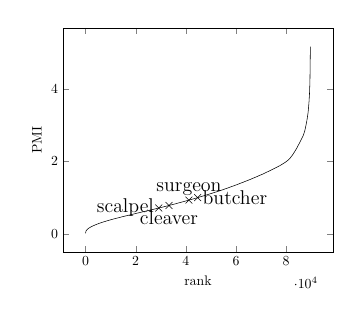
\begin{tikzpicture}[scale=0.5]
	\begin{axis} [xlabel=rank,ylabel=PMI]
	\addplot [mark=none] coordinates {
		(0,0.00622) (179,0.06993) (358,0.08958) (537,0.1038) (716,0.11612) (895,0.1277) (1074,0.13863) (1253,0.14843) (1432,0.15739) (1611,0.16389) (1790,0.17189) (1969,0.17942) (2148,0.18635) (2327,0.19268) (2506,0.19919) (2685,0.20512) (2864,0.21109) (3043,0.21663) (3222,0.22214) (3401,0.22756) (3580,0.23298) (3759,0.23843) (3938,0.24394) (4117,0.24876) (4296,0.25433) (4475,0.25886) (4654,0.26335) (4833,0.26848) (5012,0.27326) (5191,0.2776) (5370,0.28219) (5549,0.28689) (5728,0.29159) (5907,0.29576) (6086,0.29963) (6265,0.30341) (6444,0.30759) (6623,0.31191) (6802,0.31573) (6981,0.31984) (7160,0.32383) (7339,0.32767) (7518,0.33159) (7697,0.33524) (7876,0.33996) (8055,0.34371) (8234,0.34751) (8413,0.35149) (8592,0.35495) (8771,0.3588) (8950,0.36238) (9129,0.36589) (9308,0.3694) (9487,0.37303) (9666,0.37628) (9845,0.37978) (10024,0.38348) (10203,0.38663) (10382,0.39019) (10561,0.39335) (10740,0.39672) (10919,0.39989) (11098,0.40352) (11277,0.40669) (11456,0.40985) (11635,0.41317) (11814,0.41601) (11993,0.41905) (12172,0.42228) (12351,0.42574) (12530,0.42889) (12709,0.43215) (12888,0.43526) (13067,0.43861) (13246,0.44192) (13425,0.44501) (13604,0.44801) (13783,0.45097) (13962,0.45451) (14141,0.45782) (14320,0.46114) (14499,0.4642) (14678,0.46746) (14857,0.47018) (15036,0.47349) (15215,0.47674) (15394,0.47975) (15573,0.4826) (15752,0.48588) (15931,0.4887) (16110,0.49164) (16289,0.49459) (16468,0.49724) (16647,0.50011) (16826,0.50297) (17005,0.50606) (17184,0.50888) (17363,0.51207) (17542,0.51475) (17721,0.51782) (17900,0.5208) (18079,0.52378) (18258,0.52714) (18437,0.53026) (18616,0.5329) (18795,0.53599) (18974,0.53886) (19153,0.54177) (19332,0.54494) (19511,0.548) (19690,0.55123) (19869,0.55423) (20048,0.55704) (20227,0.56012) (20406,0.56341) (20585,0.56611) (20764,0.56916) (20943,0.57217) (21122,0.57508) (21301,0.57829) (21480,0.58135) (21659,0.58423) (21838,0.58723) (22017,0.59032) (22196,0.59322) (22375,0.59608) (22554,0.59926) (22733,0.60207) (22912,0.60469) (23091,0.60727) (23270,0.61001) (23449,0.61277) (23628,0.61591) (23807,0.61897) (23986,0.62215) (24165,0.6252) (24344,0.6282) (24523,0.63076) (24702,0.63338) (24881,0.63622) (25060,0.63937) (25239,0.64226) (25418,0.64501) (25597,0.64812) (25776,0.65131) (25955,0.65425) (26134,0.65743) (26313,0.66062) (26492,0.66364) (26671,0.66654) (26850,0.66942) (27029,0.67227) (27208,0.67511) (27387,0.67796) (27566,0.68096) (27745,0.68396) (27924,0.68686) (28103,0.6899) (28282,0.69294) (28461,0.69609) (28640,0.69923) (28819,0.70204) (28998,0.70543) (29177,0.70847) (29356,0.71139) (29535,0.71433) (29714,0.71735) (29893,0.71996) (30072,0.72312) (30251,0.72642) (30430,0.72947) (30609,0.7324) (30788,0.73545) (30967,0.73833) (31146,0.74182) (31325,0.74495) (31504,0.74811) (31683,0.75129) (31862,0.75405) (32041,0.75737) (32220,0.76061) (32399,0.76356) (32578,0.7666) (32757,0.76932) (32936,0.77241) (33115,0.77588) (33294,0.77932) (33473,0.78278) (33652,0.78562) (33831,0.78914) (34010,0.79218) (34189,0.79538) (34368,0.79877) (34547,0.80197) (34726,0.8054) (34905,0.80829) (35084,0.81143) (35263,0.81449) (35442,0.81771) (35621,0.82091) (35800,0.82416) (35979,0.8272) (36158,0.83062) (36337,0.83407) (36516,0.83756) (36695,0.84107) (36874,0.84487) (37053,0.84793) (37232,0.85153) (37411,0.85447) (37590,0.85752) (37769,0.86058) (37948,0.86373) (38127,0.86726) (38306,0.87084) (38485,0.87456) (38664,0.87753) (38843,0.88126) (39022,0.8846) (39201,0.88825) (39380,0.89193) (39559,0.89522) (39738,0.89852) (39917,0.90171) (40096,0.90478) (40275,0.90875) (40454,0.91248) (40633,0.91579) (40812,0.91892) (40991,0.92276) (41170,0.92593) (41349,0.92932) (41528,0.93243) (41707,0.93626) (41886,0.93965) (42065,0.94308) (42244,0.94683) (42423,0.95023) (42602,0.95332) (42781,0.95676) (42960,0.96013) (43139,0.96401) (43318,0.96757) (43497,0.97095) (43676,0.97457) (43855,0.97845) (44034,0.98163) (44213,0.98517) (44392,0.98905) (44571,0.99275) (44750,0.99655) (44929,1.0005) (45108,1.00397) (45287,1.00741) (45466,1.01108) (45645,1.01478) (45824,1.01889) (46003,1.02265) (46182,1.02606) (46361,1.02949) (46540,1.03321) (46719,1.0376) (46898,1.04151) (47077,1.04542) (47256,1.04862) (47435,1.05241) (47614,1.0561) (47793,1.06009) (47972,1.06438) (48151,1.06797) (48330,1.07158) (48509,1.07559) (48688,1.07923) (48867,1.08319) (49046,1.08722) (49225,1.09178) (49404,1.09569) (49583,1.09919) (49762,1.10272) (49941,1.10649) (50120,1.11012) (50299,1.11343) (50478,1.11751) (50657,1.12162) (50836,1.12529) (51015,1.129) (51194,1.13319) (51373,1.13788) (51552,1.14134) (51731,1.14586) (51910,1.14935) (52089,1.15353) (52268,1.15734) (52447,1.16138) (52626,1.1649) (52805,1.16941) (52984,1.17299) (53163,1.17754) (53342,1.18187) (53521,1.18572) (53700,1.18992) (53879,1.19402) (54058,1.19822) (54237,1.2028) (54416,1.20724) (54595,1.21153) (54774,1.21532) (54953,1.21968) (55132,1.22365) (55311,1.22821) (55490,1.23284) (55669,1.23688) (55848,1.24146) (56027,1.24596) (56206,1.25055) (56385,1.25462) (56564,1.25882) (56743,1.26278) (56922,1.26691) (57101,1.27167) (57280,1.27617) (57459,1.28033) (57638,1.28496) (57817,1.29007) (57996,1.29527) (58175,1.29949) (58354,1.30419) (58533,1.30862) (58712,1.31248) (58891,1.31693) (59070,1.32147) (59249,1.326) (59428,1.33084) (59607,1.33539) (59786,1.33987) (59965,1.34406) (60144,1.34878) (60323,1.35337) (60502,1.35816) (60681,1.36334) (60860,1.36826) (61039,1.37278) (61218,1.37756) (61397,1.38269) (61576,1.38757) (61755,1.39261) (61934,1.39714) (62113,1.40166) (62292,1.40597) (62471,1.41042) (62650,1.41491) (62829,1.41951) (63008,1.42551) (63187,1.4301) (63366,1.43542) (63545,1.43978) (63724,1.44486) (63903,1.45018) (64082,1.45489) (64261,1.45996) (64440,1.46479) (64619,1.46885) (64798,1.47403) (64977,1.4791) (65156,1.484) (65335,1.48895) (65514,1.49372) (65693,1.49862) (65872,1.50393) (66051,1.50995) (66230,1.51516) (66409,1.5204) (66588,1.52569) (66767,1.53057) (66946,1.5358) (67125,1.54088) (67304,1.54632) (67483,1.5512) (67662,1.55641) (67841,1.56197) (68020,1.56758) (68199,1.5728) (68378,1.57798) (68557,1.58299) (68736,1.58852) (68915,1.59337) (69094,1.59947) (69273,1.60513) (69452,1.61009) (69631,1.61542) (69810,1.62112) (69989,1.62618) (70168,1.63211) (70347,1.63643) (70526,1.6416) (70705,1.64784) (70884,1.65311) (71063,1.65867) (71242,1.66373) (71421,1.67018) (71600,1.67668) (71779,1.68261) (71958,1.68941) (72137,1.69485) (72316,1.70138) (72495,1.70665) (72674,1.71271) (72853,1.71846) (73032,1.72475) (73211,1.73033) (73390,1.73666) (73569,1.74316) (73748,1.74971) (73927,1.75572) (74106,1.76177) (74285,1.76787) (74464,1.77402) (74643,1.78022) (74822,1.78605) (75001,1.7915) (75180,1.79783) (75359,1.80407) (75538,1.80936) (75717,1.81584) (75896,1.82204) (76075,1.82837) (76254,1.83537) (76433,1.84117) (76612,1.84712) (76791,1.85413) (76970,1.86132) (77149,1.86823) (77328,1.8738) (77507,1.88035) (77686,1.88647) (77865,1.89359) (78044,1.90222) (78223,1.90897) (78402,1.91791) (78581,1.92419) (78760,1.93224) (78939,1.9403) (79118,1.94828) (79297,1.95543) (79476,1.96368) (79655,1.97165) (79834,1.98096) (80013,1.99021) (80192,1.99859) (80371,2.00809) (80550,2.01824) (80729,2.02866) (80908,2.0393) (81087,2.05115) (81266,2.06415) (81445,2.07645) (81624,2.09072) (81803,2.10798) (81982,2.12461) (82161,2.13872) (82340,2.15538) (82519,2.17155) (82698,2.19041) (82877,2.20763) (83056,2.22721) (83235,2.2473) (83414,2.26669) (83593,2.28871) (83772,2.30865) (83951,2.32968) (84130,2.35005) (84309,2.37126) (84488,2.39428) (84667,2.41776) (84846,2.44125) (85025,2.46588) (85204,2.48839) (85383,2.51048) (85562,2.5345) (85741,2.55836) (85920,2.5831) (86099,2.61013) (86278,2.63505) (86457,2.66057) (86636,2.68674) (86815,2.713) (86994,2.74309) (87173,2.78014) (87352,2.81878) (87531,2.86846) (87710,2.92534) (87889,2.98645) (88068,3.04816) (88247,3.11264) (88426,3.18631) (88605,3.2714) (88784,3.35855) (88963,3.50245) (89142,3.65465) (89321,3.85875) (89500,4.20406) (89679,5.16929)
	};
	\addplot [mark=x,only marks,mark size = 3.5] coordinates {
		(29204,0.70908)(33277,0.77903)(41247,0.92747)(44737,0.99632)
	};
	\node [anchor=east] at (axis cs: 29204,0.70908) {\Large scalpel};
	\node [anchor=north] at (axis cs: 33277,0.77903) {\Large cleaver};
	\node [anchor=south] at (axis cs: 41247,0.92747) {\Large surgeon};
	\node [anchor=west] at (axis cs: 44737,0.99632) {\Large butcher};
	\end{axis}
\end{tikzpicture}
\caption*{dimension: \emph{life}}
\end{subfigure}
\centering
\begin{subfigure} [t] {0.3 \textwidth}
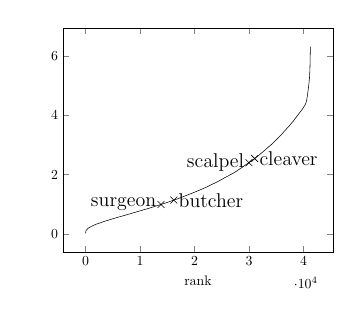
\begin{tikzpicture} [scale=0.5]
	\begin{axis} [xlabel=rank,ylabel=PMI,y label style={color=white}]
	\addplot [mark=none] coordinates {
(0,0.01004) (82,0.10112) (164,0.12417) (246,0.14062) (328,0.15755) (410,0.17296) (492,0.18456) (574,0.19468) (656,0.20589) (738,0.21453) (820,0.22473) (902,0.23274) (984,0.2401) (1066,0.24851) (1148,0.25546) (1230,0.26299) (1312,0.27054) (1394,0.27863) (1476,0.28481) (1558,0.2915) (1640,0.29752) (1722,0.30343) (1804,0.30956) (1886,0.31675) (1968,0.32333) (2050,0.32831) (2132,0.33313) (2214,0.3384) (2296,0.34394) (2378,0.34814) (2460,0.3538) (2542,0.35913) (2624,0.36444) (2706,0.36953) (2788,0.37487) (2870,0.37967) (2952,0.38513) (3034,0.38953) (3116,0.39547) (3198,0.40102) (3280,0.40585) (3362,0.41063) (3444,0.41565) (3526,0.42068) (3608,0.42616) (3690,0.4312) (3772,0.43623) (3854,0.44049) (3936,0.44462) (4018,0.44953) (4100,0.45438) (4182,0.45911) (4264,0.46431) (4346,0.46947) (4428,0.47387) (4510,0.47886) (4592,0.48422) (4674,0.48876) (4756,0.4925) (4838,0.49659) (4920,0.50107) (5002,0.50641) (5084,0.51135) (5166,0.51547) (5248,0.51932) (5330,0.52409) (5412,0.52829) (5494,0.53188) (5576,0.53712) (5658,0.5434) (5740,0.54751) (5822,0.55141) (5904,0.55585) (5986,0.56004) (6068,0.56406) (6150,0.56827) (6232,0.57183) (6314,0.57573) (6396,0.58003) (6478,0.58505) (6560,0.58909) (6642,0.5938) (6724,0.59793) (6806,0.60156) (6888,0.60534) (6970,0.61003) (7052,0.61445) (7134,0.61962) (7216,0.62455) (7298,0.62823) (7380,0.63238) (7462,0.63603) (7544,0.64026) (7626,0.64493) (7708,0.64952) (7790,0.65361) (7872,0.65815) (7954,0.66269) (8036,0.66683) (8118,0.67159) (8200,0.67607) (8282,0.67947) (8364,0.68488) (8446,0.68908) (8528,0.69304) (8610,0.69802) (8692,0.70339) (8774,0.70777) (8856,0.71124) (8938,0.71568) (9020,0.7198) (9102,0.7239) (9184,0.72878) (9266,0.73343) (9348,0.73723) (9430,0.74189) (9512,0.74635) (9594,0.75065) (9676,0.7557) (9758,0.75996) (9840,0.76391) (9922,0.76901) (10004,0.77353) (10086,0.77779) (10168,0.78219) (10250,0.78652) (10332,0.79145) (10414,0.79531) (10496,0.80012) (10578,0.80532) (10660,0.80945) (10742,0.81342) (10824,0.81732) (10906,0.82221) (10988,0.82745) (11070,0.83131) (11152,0.83563) (11234,0.83974) (11316,0.84422) (11398,0.84898) (11480,0.85286) (11562,0.85717) (11644,0.86237) (11726,0.86768) (11808,0.87183) (11890,0.8768) (11972,0.88124) (12054,0.88766) (12136,0.89174) (12218,0.89593) (12300,0.9004) (12382,0.90499) (12464,0.91022) (12546,0.91524) (12628,0.92063) (12710,0.92589) (12792,0.9302) (12874,0.93491) (12956,0.93958) (13038,0.94382) (13120,0.94897) (13202,0.95368) (13284,0.95825) (13366,0.96291) (13448,0.96773) (13530,0.97199) (13612,0.9763) (13694,0.98069) (13776,0.98459) (13858,0.98966) (13940,0.99399) (14022,0.99876) (14104,1.00333) (14186,1.00931) (14268,1.01341) (14350,1.01921) (14432,1.02376) (14514,1.02881) (14596,1.0337) (14678,1.03876) (14760,1.04444) (14842,1.04948) (14924,1.05469) (15006,1.05989) (15088,1.06474) (15170,1.06996) (15252,1.07588) (15334,1.08069) (15416,1.08643) (15498,1.09186) (15580,1.09734) (15662,1.10242) (15744,1.10785) (15826,1.11413) (15908,1.11883) (15990,1.1244) (16072,1.12913) (16154,1.13446) (16236,1.13927) (16318,1.14435) (16400,1.15018) (16482,1.15522) (16564,1.16049) (16646,1.16489) (16728,1.1701) (16810,1.17582) (16892,1.18192) (16974,1.18815) (17056,1.19322) (17138,1.19823) (17220,1.20358) (17302,1.20987) (17384,1.21516) (17466,1.21968) (17548,1.22499) (17630,1.23088) (17712,1.23803) (17794,1.24268) (17876,1.24986) (17958,1.25649) (18040,1.2622) (18122,1.26725) (18204,1.27383) (18286,1.28019) (18368,1.28526) (18450,1.29071) (18532,1.29788) (18614,1.30401) (18696,1.30931) (18778,1.31475) (18860,1.32057) (18942,1.32722) (19024,1.33404) (19106,1.33982) (19188,1.34682) (19270,1.3532) (19352,1.35828) (19434,1.36399) (19516,1.36963) (19598,1.37588) (19680,1.38155) (19762,1.38811) (19844,1.3934) (19926,1.39918) (20008,1.40595) (20090,1.41118) (20172,1.41886) (20254,1.42561) (20336,1.4322) (20418,1.43866) (20500,1.44371) (20582,1.44929) (20664,1.45499) (20746,1.46161) (20828,1.46834) (20910,1.47572) (20992,1.48208) (21074,1.48938) (21156,1.49567) (21238,1.502) (21320,1.50777) (21402,1.51482) (21484,1.52101) (21566,1.52692) (21648,1.53378) (21730,1.5405) (21812,1.54756) (21894,1.55427) (21976,1.56093) (22058,1.56736) (22140,1.57399) (22222,1.58047) (22304,1.58707) (22386,1.59404) (22468,1.60202) (22550,1.61023) (22632,1.61838) (22714,1.62572) (22796,1.63352) (22878,1.64017) (22960,1.6482) (23042,1.65694) (23124,1.66455) (23206,1.66957) (23288,1.67764) (23370,1.68445) (23452,1.69159) (23534,1.69743) (23616,1.7047) (23698,1.71182) (23780,1.71945) (23862,1.72803) (23944,1.73609) (24026,1.74283) (24108,1.74953) (24190,1.75746) (24272,1.76496) (24354,1.77295) (24436,1.7803) (24518,1.78909) (24600,1.79816) (24682,1.80732) (24764,1.81569) (24846,1.82402) (24928,1.83185) (25010,1.83983) (25092,1.84653) (25174,1.85539) (25256,1.86431) (25338,1.87298) (25420,1.88129) (25502,1.89292) (25584,1.90107) (25666,1.90717) (25748,1.91474) (25830,1.92326) (25912,1.93098) (25994,1.93822) (26076,1.94552) (26158,1.95458) (26240,1.96421) (26322,1.97138) (26404,1.98058) (26486,1.98953) (26568,1.99806) (26650,2.0048) (26732,2.01379) (26814,2.02163) (26896,2.03003) (26978,2.0378) (27060,2.04688) (27142,2.05528) (27224,2.06416) (27306,2.0726) (27388,2.08179) (27470,2.09186) (27552,2.1006) (27634,2.11046) (27716,2.11894) (27798,2.12917) (27880,2.14078) (27962,2.15169) (28044,2.16215) (28126,2.17069) (28208,2.18003) (28290,2.1901) (28372,2.20237) (28454,2.21281) (28536,2.22127) (28618,2.23267) (28700,2.24393) (28782,2.25311) (28864,2.26285) (28946,2.27433) (29028,2.28413) (29110,2.29509) (29192,2.30673) (29274,2.31722) (29356,2.3273) (29438,2.3381) (29520,2.34938) (29602,2.35963) (29684,2.36963) (29766,2.37996) (29848,2.38884) (29930,2.39786) (30012,2.40662) (30094,2.41785) (30176,2.42997) (30258,2.43904) (30340,2.44846) (30422,2.45941) (30504,2.47207) (30586,2.48308) (30668,2.49381) (30750,2.50379) (30832,2.51552) (30914,2.5269) (30996,2.53916) (31078,2.55115) (31160,2.56154) (31242,2.57291) (31324,2.58307) (31406,2.59604) (31488,2.60689) (31570,2.61998) (31652,2.63238) (31734,2.64579) (31816,2.65861) (31898,2.67144) (31980,2.68472) (32062,2.69803) (32144,2.712) (32226,2.72464) (32308,2.73657) (32390,2.74777) (32472,2.75953) (32554,2.77461) (32636,2.78639) (32718,2.79994) (32800,2.81118) (32882,2.82421) (32964,2.83656) (33046,2.84961) (33128,2.8645) (33210,2.87854) (33292,2.89033) (33374,2.90405) (33456,2.91733) (33538,2.92832) (33620,2.94034) (33702,2.95501) (33784,2.96828) (33866,2.98301) (33948,2.99515) (34030,3.00776) (34112,3.02234) (34194,3.03712) (34276,3.05141) (34358,3.06588) (34440,3.07913) (34522,3.09254) (34604,3.10971) (34686,3.12494) (34768,3.1389) (34850,3.15573) (34932,3.16772) (35014,3.17953) (35096,3.19689) (35178,3.20979) (35260,3.22681) (35342,3.24166) (35424,3.25793) (35506,3.27277) (35588,3.28864) (35670,3.30331) (35752,3.32018) (35834,3.33539) (35916,3.34992) (35998,3.36567) (36080,3.38042) (36162,3.39874) (36244,3.42298) (36326,3.43814) (36408,3.45543) (36490,3.472) (36572,3.48727) (36654,3.50482) (36736,3.5231) (36818,3.53751) (36900,3.55525) (36982,3.57058) (37064,3.58827) (37146,3.60348) (37228,3.6211) (37310,3.63785) (37392,3.6537) (37474,3.67321) (37556,3.69422) (37638,3.70843) (37720,3.72642) (37802,3.74467) (37884,3.76195) (37966,3.782) (38048,3.79854) (38130,3.81529) (38212,3.83622) (38294,3.85617) (38376,3.8778) (38458,3.89704) (38540,3.91657) (38622,3.93641) (38704,3.95512) (38786,3.97558) (38868,3.99189) (38950,4.01043) (39032,4.03438) (39114,4.05616) (39196,4.07354) (39278,4.09439) (39360,4.11559) (39442,4.13547) (39524,4.15566) (39606,4.17789) (39688,4.19701) (39770,4.21642) (39852,4.23612) (39934,4.25803) (40016,4.28428) (40098,4.31039) (40180,4.33158) (40262,4.35509) (40344,4.38619) (40426,4.42515) (40508,4.47456) (40590,4.55117) (40672,4.63453) (40754,4.74044) (40836,4.86945) (40918,4.977) (41000,5.1181) (41082,5.27117) (41164,5.55781) (41246,6.33026)
	};
	\addplot [mark=x,only marks,mark size = 3.5] coordinates {
		(13845,0.98899)(16190,1.13695)(29968,2.40174)(31024,2.54414)
	};
	\node [anchor=east] at (axis cs: 13845,0.98899) {\Large surgeon};
	\node [anchor=west] at (axis cs: 16190,1.13695) {\Large butcher};
	\node [anchor=east] at (axis cs: 29968,2.40174) {\Large scalpel};
	\node [anchor=west] at (axis cs: 31024,2.54414) {\Large cleaver};
	\end{axis}
\end{tikzpicture}
\caption*{dimension: \emph{hands}}
\end{subfigure}
\centering
\begin{subfigure} [t] {0.3 \textwidth}
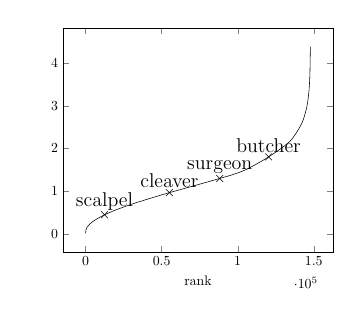
\begin{tikzpicture} [scale=0.5]
	\begin{axis} [xlabel=rank,ylabel=PMI,y label style={color=white}]
	\addplot [mark=none] coordinates {
		(0,0.00873) (295,0.08756) (590,0.12013) (885,0.14286) (1180,0.1607) (1475,0.17372) (1770,0.18662) (2065,0.20012) (2360,0.21206) (2655,0.22349) (2950,0.23441) (3245,0.24433) (3540,0.25194) (3835,0.26042) (4130,0.26934) (4425,0.27875) (4720,0.28699) (5015,0.29465) (5310,0.30183) (5605,0.30913) (5900,0.31561) (6195,0.32201) (6490,0.32861) (6785,0.33471) (7080,0.3407) (7375,0.3472) (7670,0.35305) (7965,0.35943) (8260,0.36555) (8555,0.37194) (8850,0.37792) (9145,0.38409) (9440,0.38982) (9735,0.39532) (10030,0.40097) (10325,0.4068) (10620,0.41244) (10915,0.4175) (11210,0.42332) (11505,0.4289) (11800,0.43381) (12095,0.43959) (12390,0.44398) (12685,0.44896) (12980,0.45406) (13275,0.45911) (13570,0.4639) (13865,0.46904) (14160,0.47337) (14455,0.47822) (14750,0.48215) (15045,0.48676) (15340,0.49105) (15635,0.4958) (15930,0.50037) (16225,0.50464) (16520,0.50927) (16815,0.51314) (17110,0.5178) (17405,0.5226) (17700,0.52745) (17995,0.53188) (18290,0.53667) (18585,0.54042) (18880,0.54459) (19175,0.54871) (19470,0.55311) (19765,0.55732) (20060,0.56142) (20355,0.56567) (20650,0.5698) (20945,0.57383) (21240,0.57791) (21535,0.58164) (21830,0.58552) (22125,0.58925) (22420,0.59313) (22715,0.59699) (23010,0.60082) (23305,0.60506) (23600,0.60903) (23895,0.61294) (24190,0.61639) (24485,0.62025) (24780,0.62395) (25075,0.62797) (25370,0.6315) (25665,0.63521) (25960,0.63898) (26255,0.64253) (26550,0.64675) (26845,0.65017) (27140,0.65398) (27435,0.65793) (27730,0.66142) (28025,0.66484) (28320,0.66857) (28615,0.67248) (28910,0.67612) (29205,0.67968) (29500,0.68328) (29795,0.68728) (30090,0.69088) (30385,0.69415) (30680,0.69775) (30975,0.70109) (31270,0.70435) (31565,0.70817) (31860,0.71161) (32155,0.71545) (32450,0.71891) (32745,0.72262) (33040,0.72637) (33335,0.72966) (33630,0.7331) (33925,0.73667) (34220,0.73973) (34515,0.74279) (34810,0.7459) (35105,0.74919) (35400,0.75252) (35695,0.75606) (35990,0.75912) (36285,0.76252) (36580,0.76565) (36875,0.76909) (37170,0.7723) (37465,0.77577) (37760,0.77899) (38055,0.78258) (38350,0.78613) (38645,0.78925) (38940,0.79236) (39235,0.79558) (39530,0.79895) (39825,0.80261) (40120,0.80618) (40415,0.8093) (40710,0.81259) (41005,0.81587) (41300,0.8189) (41595,0.822) (41890,0.82529) (42185,0.82836) (42480,0.831) (42775,0.8342) (43070,0.83738) (43365,0.84046) (43660,0.84368) (43955,0.84705) (44250,0.8503) (44545,0.8539) (44840,0.8571) (45135,0.86037) (45430,0.8634) (45725,0.86668) (46020,0.86967) (46315,0.87284) (46610,0.87596) (46905,0.87934) (47200,0.88226) (47495,0.88532) (47790,0.88815) (48085,0.89148) (48380,0.89464) (48675,0.89792) (48970,0.90121) (49265,0.90408) (49560,0.90712) (49855,0.9105) (50150,0.91355) (50445,0.91662) (50740,0.9196) (51035,0.92264) (51330,0.92587) (51625,0.92858) (51920,0.9317) (52215,0.93476) (52510,0.93752) (52805,0.94067) (53100,0.94403) (53395,0.94684) (53690,0.94973) (53985,0.9531) (54280,0.95608) (54575,0.95903) (54870,0.96235) (55165,0.96528) (55460,0.96823) (55755,0.9709) (56050,0.97389) (56345,0.97714) (56640,0.98012) (56935,0.98296) (57230,0.98571) (57525,0.98879) (57820,0.99174) (58115,0.99439) (58410,0.99753) (58705,1.00047) (59000,1.00323) (59295,1.00594) (59590,1.00932) (59885,1.01223) (60180,1.01548) (60475,1.01823) (60770,1.02118) (61065,1.02405) (61360,1.02711) (61655,1.03007) (61950,1.03277) (62245,1.03554) (62540,1.03864) (62835,1.04148) (63130,1.04441) (63425,1.04769) (63720,1.05068) (64015,1.05349) (64310,1.05632) (64605,1.05917) (64900,1.06239) (65195,1.06491) (65490,1.06798) (65785,1.071) (66080,1.07403) (66375,1.07658) (66670,1.07991) (66965,1.08284) (67260,1.08551) (67555,1.08852) (67850,1.09125) (68145,1.09441) (68440,1.09761) (68735,1.10049) (69030,1.10307) (69325,1.10642) (69620,1.10932) (69915,1.11248) (70210,1.11485) (70505,1.11804) (70800,1.12124) (71095,1.12447) (71390,1.12701) (71685,1.13009) (71980,1.13278) (72275,1.13605) (72570,1.13922) (72865,1.14204) (73160,1.14507) (73455,1.1477) (73750,1.15088) (74045,1.15353) (74340,1.15627) (74635,1.15954) (74930,1.16242) (75225,1.16531) (75520,1.16823) (75815,1.17134) (76110,1.17439) (76405,1.17706) (76700,1.18063) (76995,1.18332) (77290,1.18603) (77585,1.18921) (77880,1.19209) (78175,1.19502) (78470,1.19791) (78765,1.20069) (79060,1.20348) (79355,1.20629) (79650,1.20911) (79945,1.21241) (80240,1.21555) (80535,1.21861) (80830,1.22149) (81125,1.22487) (81420,1.22827) (81715,1.2312) (82010,1.23414) (82305,1.2371) (82600,1.24007) (82895,1.24306) (83190,1.24607) (83485,1.24909) (83780,1.25212) (84075,1.25535) (84370,1.25824) (84665,1.26133) (84960,1.26442) (85255,1.26754) (85550,1.27015) (85845,1.27382) (86140,1.27646) (86435,1.27964) (86730,1.28301) (87025,1.28595) (87320,1.28874) (87615,1.29198) (87910,1.29524) (88205,1.29761) (88500,1.30072) (88795,1.3032) (89090,1.30647) (89385,1.30959) (89680,1.31294) (89975,1.31632) (90270,1.31929) (90565,1.32248) (90860,1.32542) (91155,1.32867) (91450,1.3314) (91745,1.33452) (92040,1.33719) (92335,1.34049) (92630,1.34284) (92925,1.34614) (93220,1.34875) (93515,1.35203) (93810,1.35513) (94105,1.35834) (94400,1.36124) (94695,1.3644) (94990,1.36758) (95285,1.37061) (95580,1.37423) (95875,1.37795) (96170,1.38107) (96465,1.38484) (96760,1.38799) (97055,1.39179) (97350,1.3951) (97645,1.39904) (97940,1.40205) (98235,1.40594) (98530,1.40985) (98825,1.41309) (99120,1.41642) (99415,1.42032) (99710,1.4238) (100005,1.42707) (100300,1.43096) (100595,1.43467) (100890,1.4381) (101185,1.44215) (101480,1.44614) (101775,1.4503) (102070,1.45448) (102365,1.45869) (102660,1.46256) (102955,1.46711) (103250,1.47148) (103545,1.4758) (103840,1.48063) (104135,1.48506) (104430,1.4899) (104725,1.49483) (105020,1.4993) (105315,1.50405) (105610,1.50883) (105905,1.51364) (106200,1.51823) (106495,1.52355) (106790,1.52829) (107085,1.5334) (107380,1.53849) (107675,1.54404) (107970,1.54991) (108265,1.55528) (108560,1.56097) (108855,1.56671) (109150,1.57221) (109445,1.57817) (109740,1.58419) (110035,1.58962) (110330,1.59523) (110625,1.60124) (110920,1.60644) (111215,1.6124) (111510,1.61807) (111805,1.62349) (112100,1.62939) (112395,1.63614) (112690,1.64192) (112985,1.64777) (113280,1.65342) (113575,1.65958) (113870,1.6656) (114165,1.6715) (114460,1.67753) (114755,1.68362) (115050,1.69056) (115345,1.69642) (115640,1.70314) (115935,1.70894) (116230,1.71511) (116525,1.72116) (116820,1.72726) (117115,1.7334) (117410,1.7396) (117705,1.7455) (118000,1.75179) (118295,1.75814) (118590,1.76493) (118885,1.77188) (119180,1.77858) (119475,1.78441) (119770,1.79103) (120065,1.7977) (120360,1.8048) (120655,1.81196) (120950,1.81804) (121245,1.82571) (121540,1.83226) (121835,1.83877) (122130,1.84628) (122425,1.85314) (122720,1.85995) (123015,1.86691) (123310,1.87338) (123605,1.8807) (123900,1.88815) (124195,1.89467) (124490,1.90165) (124785,1.90879) (125080,1.91606) (125375,1.92384) (125670,1.93038) (125965,1.93784) (126260,1.94493) (126555,1.95164) (126850,1.95975) (127145,1.96748) (127440,1.97439) (127735,1.9813) (128030,1.98876) (128325,1.99629) (128620,2.00293) (128915,2.0101) (129210,2.0185) (129505,2.02609) (129800,2.0342) (130095,2.04288) (130390,2.05098) (130685,2.05863) (130980,2.06739) (131275,2.07588) (131570,2.08472) (131865,2.09207) (132160,2.10107) (132455,2.11016) (132750,2.11881) (133045,2.12863) (133340,2.13745) (133635,2.14679) (133930,2.15536) (134225,2.16597) (134520,2.17709) (134815,2.1879) (135110,2.20013) (135405,2.21217) (135700,2.22397) (135995,2.23776) (136290,2.25101) (136585,2.26502) (136880,2.28041) (137175,2.29604) (137470,2.3102) (137765,2.32542) (138060,2.3402) (138355,2.35664) (138650,2.37329) (138945,2.38835) (139240,2.40539) (139535,2.42262) (139830,2.43996) (140125,2.45796) (140420,2.47517) (140715,2.49428) (141010,2.51376) (141305,2.53363) (141600,2.55316) (141895,2.57224) (142190,2.59489) (142485,2.6199) (142780,2.6466) (143075,2.67209) (143370,2.70154) (143665,2.73407) (143960,2.77034) (144255,2.80907) (144550,2.84553) (144845,2.88325) (145140,2.92826) (145435,2.97315) (145730,3.03039) (146025,3.09462) (146320,3.17092) (146615,3.25689) (146910,3.36659) (147205,3.52351) (147500,3.75669) (147795,4.38804)
	};
	\addplot [mark=x,only marks,mark size = 3.5] coordinates {
		(12466,0.44529)(55096,0.9647)(88206,1.29763)(120293,1.80307)
	};
	\node [anchor=south] at (axis cs: 12466,0.44529) {\Large scalpel};
	\node [anchor=south] at (axis cs: 55096,0.9647) {\Large cleaver};
	\node [anchor=south] at (axis cs: 88206,1.29763) {\Large surgeon};
	\node [anchor=south] at (axis cs: 120293,1.80307) {\Large butcher};
	\end{axis}
\end{tikzpicture}
\caption*{dimension: \emph{known}}
\end{subfigure}
\caption{\textsc{surgery} $\Longleftrightarrow$ \textsc{butchery}}
\vspace{0.5cm}
\end{subfigure}
\begin{subfigure} {1 \textwidth}
\centering
\begin{subfigure} [t] {0.3 \textwidth}
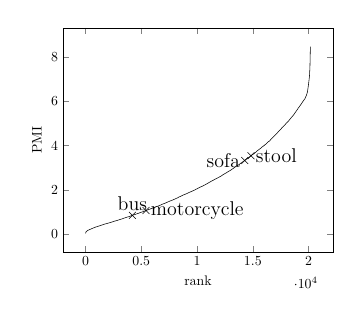
\begin{tikzpicture}[scale=0.5]
	\begin{axis} [xlabel=rank,ylabel=PMI]
	\addplot [mark=none] coordinates {
		(0,0.01807) (40,0.08801) (80,0.10418) (120,0.12301) (160,0.14129) (200,0.15581) (240,0.16573) (280,0.17348) (320,0.18302) (360,0.19209) (400,0.19925) (440,0.20666) (480,0.21617) (520,0.22443) (560,0.23427) (600,0.24492) (640,0.2522) (680,0.25943) (720,0.26829) (760,0.27649) (800,0.28612) (840,0.29261) (880,0.30053) (920,0.3083) (960,0.31429) (1000,0.32115) (1040,0.32744) (1080,0.33394) (1120,0.33954) (1160,0.34584) (1200,0.35315) (1240,0.36033) (1280,0.36684) (1320,0.37535) (1360,0.38349) (1400,0.38811) (1440,0.39368) (1480,0.40195) (1520,0.40817) (1560,0.41464) (1600,0.42235) (1640,0.42853) (1680,0.4332) (1720,0.43933) (1760,0.44643) (1800,0.45126) (1840,0.45798) (1880,0.46196) (1920,0.46764) (1960,0.47397) (2000,0.47976) (2040,0.48468) (2080,0.48959) (2120,0.49501) (2160,0.50245) (2200,0.50999) (2240,0.51565) (2280,0.52219) (2320,0.5278) (2360,0.53419) (2400,0.54039) (2440,0.54867) (2480,0.55612) (2520,0.56246) (2560,0.56867) (2600,0.57441) (2640,0.5796) (2680,0.58426) (2720,0.58904) (2760,0.59574) (2800,0.60044) (2840,0.60746) (2880,0.61395) (2920,0.62132) (2960,0.62723) (3000,0.63414) (3040,0.64035) (3080,0.64664) (3120,0.65309) (3160,0.65962) (3200,0.66545) (3240,0.67194) (3280,0.67898) (3320,0.68574) (3360,0.69314) (3400,0.70106) (3440,0.70755) (3480,0.71562) (3520,0.7207) (3560,0.72882) (3600,0.73589) (3640,0.74281) (3680,0.74879) (3720,0.7544) (3760,0.76031) (3800,0.76655) (3840,0.77243) (3880,0.77811) (3920,0.78593) (3960,0.79245) (4000,0.79987) (4040,0.80729) (4080,0.8142) (4120,0.82146) (4160,0.82796) (4200,0.83549) (4240,0.84197) (4280,0.84908) (4320,0.85632) (4360,0.86174) (4400,0.86933) (4440,0.8756) (4480,0.88284) (4520,0.89014) (4560,0.89881) (4600,0.90487) (4640,0.91227) (4680,0.91933) (4720,0.92417) (4760,0.93282) (4800,0.94148) (4840,0.94876) (4880,0.95675) (4920,0.96371) (4960,0.97209) (5000,0.97936) (5040,0.98524) (5080,0.99071) (5120,0.99736) (5160,1.00528) (5200,1.01284) (5240,1.02125) (5280,1.02867) (5320,1.03627) (5360,1.04287) (5400,1.05073) (5440,1.05861) (5480,1.06603) (5520,1.07379) (5560,1.08193) (5600,1.08765) (5640,1.09719) (5680,1.10606) (5720,1.11176) (5760,1.11926) (5800,1.12635) (5840,1.13377) (5880,1.14269) (5920,1.14935) (5960,1.15627) (6000,1.1636) (6040,1.1701) (6080,1.17731) (6120,1.18418) (6160,1.19197) (6200,1.1989) (6240,1.20822) (6280,1.21744) (6320,1.22496) (6360,1.23316) (6400,1.23927) (6440,1.24692) (6480,1.25445) (6520,1.26039) (6560,1.26904) (6600,1.27511) (6640,1.28492) (6680,1.29403) (6720,1.30086) (6760,1.31208) (6800,1.32188) (6840,1.32958) (6880,1.33859) (6920,1.34533) (6960,1.35409) (7000,1.36271) (7040,1.37123) (7080,1.37765) (7120,1.38479) (7160,1.39208) (7200,1.40575) (7240,1.41438) (7280,1.42119) (7320,1.43062) (7360,1.4395) (7400,1.44675) (7440,1.45623) (7480,1.46539) (7520,1.47414) (7560,1.48473) (7600,1.49235) (7640,1.49913) (7680,1.50652) (7720,1.51479) (7760,1.52353) (7800,1.53037) (7840,1.53949) (7880,1.54613) (7920,1.55628) (7960,1.56419) (8000,1.57432) (8040,1.58193) (8080,1.59268) (8120,1.60133) (8160,1.61242) (8200,1.61978) (8240,1.6293) (8280,1.63936) (8320,1.65024) (8360,1.66408) (8400,1.67438) (8440,1.68316) (8480,1.69048) (8520,1.69936) (8560,1.71055) (8600,1.72011) (8640,1.72834) (8680,1.73853) (8720,1.74845) (8760,1.76032) (8800,1.76736) (8840,1.7744) (8880,1.78424) (8920,1.79016) (8960,1.79683) (9000,1.80609) (9040,1.81228) (9080,1.82274) (9120,1.83172) (9160,1.8421) (9200,1.85209) (9240,1.86091) (9280,1.87269) (9320,1.88162) (9360,1.88979) (9400,1.89826) (9440,1.90599) (9480,1.91318) (9520,1.92505) (9560,1.93444) (9600,1.94571) (9640,1.95504) (9680,1.9624) (9720,1.97049) (9760,1.98027) (9800,1.98918) (9840,2.0016) (9880,2.00995) (9920,2.02339) (9960,2.03356) (10000,2.04012) (10040,2.05054) (10080,2.06164) (10120,2.07297) (10160,2.08342) (10200,2.0928) (10240,2.10547) (10280,2.11516) (10320,2.12376) (10360,2.13386) (10400,2.1439) (10440,2.15238) (10480,2.16081) (10520,2.17133) (10560,2.18265) (10600,2.19398) (10640,2.20381) (10680,2.21223) (10720,2.22306) (10760,2.23474) (10800,2.24643) (10840,2.25555) (10880,2.26544) (10920,2.27881) (10960,2.29083) (11000,2.30002) (11040,2.31485) (11080,2.32973) (11120,2.3392) (11160,2.3485) (11200,2.36166) (11240,2.37261) (11280,2.38412) (11320,2.39335) (11360,2.40443) (11400,2.41346) (11440,2.4227) (11480,2.43726) (11520,2.44936) (11560,2.45841) (11600,2.47049) (11640,2.48135) (11680,2.49211) (11720,2.50352) (11760,2.51282) (11800,2.52109) (11840,2.53395) (11880,2.545) (11920,2.55443) (11960,2.56242) (12000,2.57606) (12040,2.58694) (12080,2.59861) (12120,2.60894) (12160,2.61961) (12200,2.63369) (12240,2.64586) (12280,2.66221) (12320,2.67431) (12360,2.69066) (12400,2.6994) (12440,2.71171) (12480,2.72202) (12520,2.73614) (12560,2.74619) (12600,2.75654) (12640,2.76956) (12680,2.78287) (12720,2.79596) (12760,2.80968) (12800,2.81987) (12840,2.83228) (12880,2.84536) (12920,2.85678) (12960,2.86698) (13000,2.87818) (13040,2.89375) (13080,2.90522) (13120,2.92417) (13160,2.93753) (13200,2.94947) (13240,2.96012) (13280,2.97727) (13320,2.9919) (13360,3.00949) (13400,3.02117) (13440,3.03374) (13480,3.04755) (13520,3.05834) (13560,3.07082) (13600,3.0871) (13640,3.10039) (13680,3.10995) (13720,3.12238) (13760,3.13939) (13800,3.15244) (13840,3.16883) (13880,3.18291) (13920,3.20048) (13960,3.21259) (14000,3.22557) (14040,3.23974) (14080,3.25826) (14120,3.27274) (14160,3.28916) (14200,3.30187) (14240,3.31464) (14280,3.32685) (14320,3.34422) (14360,3.35955) (14400,3.37416) (14440,3.38942) (14480,3.40227) (14520,3.41754) (14560,3.43544) (14600,3.4499) (14640,3.46429) (14680,3.48082) (14720,3.49309) (14760,3.50882) (14800,3.52889) (14840,3.54133) (14880,3.55606) (14920,3.57191) (14960,3.58483) (15000,3.59644) (15040,3.6079) (15080,3.62025) (15120,3.63744) (15160,3.65677) (15200,3.67548) (15240,3.69116) (15280,3.7069) (15320,3.72407) (15360,3.74242) (15400,3.76264) (15440,3.77522) (15480,3.79392) (15520,3.80815) (15560,3.823) (15600,3.83745) (15640,3.85162) (15680,3.86861) (15720,3.88566) (15760,3.90269) (15800,3.92281) (15840,3.93808) (15880,3.95319) (15920,3.96735) (15960,3.98367) (16000,3.99655) (16040,4.01665) (16080,4.03154) (16120,4.04681) (16160,4.06307) (16200,4.08056) (16240,4.09747) (16280,4.11544) (16320,4.13794) (16360,4.16041) (16400,4.17619) (16440,4.18668) (16480,4.20069) (16520,4.21994) (16560,4.24088) (16600,4.27185) (16640,4.29437) (16680,4.31532) (16720,4.3308) (16760,4.35218) (16800,4.37409) (16840,4.39314) (16880,4.41213) (16920,4.43346) (16960,4.45623) (17000,4.47329) (17040,4.49395) (17080,4.5178) (17120,4.53568) (17160,4.55734) (17200,4.57458) (17240,4.59707) (17280,4.62703) (17320,4.64836) (17360,4.66724) (17400,4.68684) (17440,4.70584) (17480,4.72579) (17520,4.74673) (17560,4.77423) (17600,4.80443) (17640,4.82303) (17680,4.84336) (17720,4.86325) (17760,4.87968) (17800,4.89859) (17840,4.91932) (17880,4.93802) (17920,4.96176) (17960,4.98855) (18000,5.01136) (18040,5.03271) (18080,5.04927) (18120,5.06802) (18160,5.08802) (18200,5.11516) (18240,5.13573) (18280,5.16277) (18320,5.18799) (18360,5.21535) (18400,5.23597) (18440,5.26559) (18480,5.2857) (18520,5.31125) (18560,5.33205) (18600,5.35544) (18640,5.3811) (18680,5.40519) (18720,5.43988) (18760,5.46503) (18800,5.50009) (18840,5.52036) (18880,5.55379) (18920,5.58679) (18960,5.60966) (19000,5.63683) (19040,5.66454) (19080,5.70512) (19120,5.72745) (19160,5.75436) (19200,5.78418) (19240,5.81058) (19280,5.84203) (19320,5.86725) (19360,5.89922) (19400,5.92953) (19440,5.95886) (19480,5.99326) (19520,6.01635) (19560,6.04723) (19600,6.07737) (19640,6.09996) (19680,6.13968) (19720,6.17574) (19760,6.22564) (19800,6.27326) (19840,6.32788) (19880,6.40042) (19920,6.51553) (19960,6.64487) (20000,6.80067) (20040,6.97572) (20080,7.15608) (20120,7.55856) (20160,8.4825)
	};
	\addplot [mark=x,only marks,mark size = 3.5] coordinates {
		(4203,0.83647)(5424,1.05531)(14277,3.32574)(14839,3.5408)
	};
	\node [anchor=south] at (axis cs: 4203,0.83647) {\Large bus};
	\node [anchor=west] at (axis cs: 5424,1.05531) {\Large motorcycle};
	\node [anchor=east] at (axis cs: 14277,3.32574) {\Large sofa};
	\node [anchor=west] at (axis cs: 14839,3.5408) {\Large stool};
	\end{axis}
\end{tikzpicture}
\caption*{dimension: \emph{beneath}}
\end{subfigure}
\centering
\begin{subfigure} [t] {0.3 \textwidth}
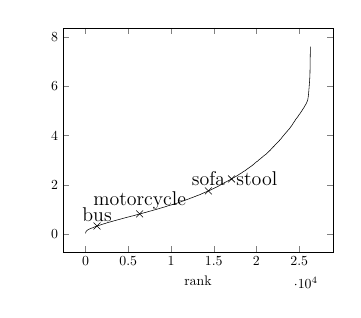
\begin{tikzpicture} [scale=0.5]
	\begin{axis} [xlabel=rank,ylabel=PMI,y label style={color=white}]
	\addplot [mark=none] coordinates {
(0,0.01675) (52,0.08641) (104,0.11395) (156,0.13152) (208,0.1449) (260,0.15729) (312,0.17009) (364,0.17929) (416,0.18943) (468,0.1969) (520,0.20568) (572,0.2132) (624,0.21885) (676,0.22786) (728,0.23473) (780,0.24152) (832,0.24796) (884,0.25543) (936,0.26243) (988,0.27045) (1040,0.27913) (1092,0.28643) (1144,0.29415) (1196,0.30079) (1248,0.30665) (1300,0.31381) (1352,0.31869) (1404,0.32553) (1456,0.32988) (1508,0.33585) (1560,0.34145) (1612,0.34818) (1664,0.35317) (1716,0.35886) (1768,0.36514) (1820,0.37003) (1872,0.37564) (1924,0.3832) (1976,0.39085) (2028,0.39488) (2080,0.4006) (2132,0.40667) (2184,0.41182) (2236,0.4179) (2288,0.42295) (2340,0.42819) (2392,0.43405) (2444,0.43963) (2496,0.44618) (2548,0.45159) (2600,0.45816) (2652,0.46318) (2704,0.46832) (2756,0.47341) (2808,0.47754) (2860,0.48276) (2912,0.48842) (2964,0.49329) (3016,0.49825) (3068,0.50391) (3120,0.50884) (3172,0.51291) (3224,0.5187) (3276,0.52385) (3328,0.52874) (3380,0.5338) (3432,0.53903) (3484,0.54366) (3536,0.54937) (3588,0.55397) (3640,0.55857) (3692,0.56373) (3744,0.56811) (3796,0.5727) (3848,0.57747) (3900,0.58307) (3952,0.5891) (4004,0.59307) (4056,0.59741) (4108,0.60246) (4160,0.60724) (4212,0.61081) (4264,0.61717) (4316,0.62245) (4368,0.62751) (4420,0.63213) (4472,0.63629) (4524,0.6414) (4576,0.64775) (4628,0.6524) (4680,0.65749) (4732,0.66224) (4784,0.66706) (4836,0.67126) (4888,0.67651) (4940,0.68154) (4992,0.68524) (5044,0.68999) (5096,0.69385) (5148,0.69916) (5200,0.70293) (5252,0.70693) (5304,0.71355) (5356,0.71872) (5408,0.72332) (5460,0.72674) (5512,0.73123) (5564,0.73429) (5616,0.73977) (5668,0.74452) (5720,0.75034) (5772,0.75588) (5824,0.76084) (5876,0.76676) (5928,0.7713) (5980,0.77605) (6032,0.78111) (6084,0.78565) (6136,0.79083) (6188,0.79523) (6240,0.80015) (6292,0.8061) (6344,0.81023) (6396,0.81556) (6448,0.81937) (6500,0.82353) (6552,0.82768) (6604,0.83212) (6656,0.83751) (6708,0.84267) (6760,0.84799) (6812,0.85396) (6864,0.85863) (6916,0.86424) (6968,0.86889) (7020,0.8725) (7072,0.87776) (7124,0.88178) (7176,0.88732) (7228,0.89208) (7280,0.89809) (7332,0.90496) (7384,0.90931) (7436,0.91509) (7488,0.91987) (7540,0.92362) (7592,0.92844) (7644,0.93292) (7696,0.93776) (7748,0.94194) (7800,0.94755) (7852,0.95238) (7904,0.95773) (7956,0.96306) (8008,0.97007) (8060,0.97382) (8112,0.97951) (8164,0.98387) (8216,0.98935) (8268,0.99435) (8320,0.9995) (8372,1.00407) (8424,1.00961) (8476,1.01384) (8528,1.02025) (8580,1.02592) (8632,1.03259) (8684,1.03735) (8736,1.0435) (8788,1.0487) (8840,1.05465) (8892,1.06012) (8944,1.06401) (8996,1.07007) (9048,1.07441) (9100,1.07969) (9152,1.0847) (9204,1.09) (9256,1.09604) (9308,1.10209) (9360,1.10758) (9412,1.11374) (9464,1.11928) (9516,1.12455) (9568,1.13098) (9620,1.13692) (9672,1.14262) (9724,1.14858) (9776,1.1536) (9828,1.15842) (9880,1.16313) (9932,1.16853) (9984,1.17291) (10036,1.17854) (10088,1.18346) (10140,1.18852) (10192,1.19436) (10244,1.199) (10296,1.20414) (10348,1.20985) (10400,1.21496) (10452,1.22073) (10504,1.22604) (10556,1.23157) (10608,1.23724) (10660,1.24303) (10712,1.2509) (10764,1.25676) (10816,1.26352) (10868,1.26996) (10920,1.27608) (10972,1.28217) (11024,1.28931) (11076,1.2969) (11128,1.30266) (11180,1.30913) (11232,1.31495) (11284,1.3221) (11336,1.32859) (11388,1.33513) (11440,1.33995) (11492,1.34681) (11544,1.35484) (11596,1.36172) (11648,1.3687) (11700,1.37499) (11752,1.38126) (11804,1.38807) (11856,1.39423) (11908,1.40122) (11960,1.40758) (12012,1.41314) (12064,1.41881) (12116,1.42723) (12168,1.43483) (12220,1.4424) (12272,1.45004) (12324,1.45626) (12376,1.46225) (12428,1.46947) (12480,1.47682) (12532,1.48399) (12584,1.49058) (12636,1.49646) (12688,1.50401) (12740,1.51107) (12792,1.51755) (12844,1.52406) (12896,1.53161) (12948,1.54055) (13000,1.54726) (13052,1.55481) (13104,1.56229) (13156,1.56842) (13208,1.57561) (13260,1.58041) (13312,1.58707) (13364,1.59383) (13416,1.60063) (13468,1.60916) (13520,1.61841) (13572,1.62766) (13624,1.63437) (13676,1.64123) (13728,1.64889) (13780,1.65654) (13832,1.66581) (13884,1.67465) (13936,1.68224) (13988,1.68884) (14040,1.6962) (14092,1.70327) (14144,1.71105) (14196,1.71988) (14248,1.72675) (14300,1.73522) (14352,1.74508) (14404,1.75366) (14456,1.76129) (14508,1.76854) (14560,1.77598) (14612,1.78352) (14664,1.79208) (14716,1.79963) (14768,1.81081) (14820,1.81956) (14872,1.82727) (14924,1.83641) (14976,1.84516) (15028,1.85275) (15080,1.86176) (15132,1.87215) (15184,1.88023) (15236,1.8889) (15288,1.89521) (15340,1.90477) (15392,1.91482) (15444,1.92311) (15496,1.93267) (15548,1.94245) (15600,1.95205) (15652,1.96163) (15704,1.97043) (15756,1.98125) (15808,1.99479) (15860,2.00513) (15912,2.01522) (15964,2.02509) (16016,2.03434) (16068,2.04523) (16120,2.05538) (16172,2.06331) (16224,2.0722) (16276,2.08273) (16328,2.09225) (16380,2.1047) (16432,2.11348) (16484,2.12113) (16536,2.13223) (16588,2.14104) (16640,2.15074) (16692,2.15914) (16744,2.16867) (16796,2.17831) (16848,2.18905) (16900,2.19981) (16952,2.20986) (17004,2.22016) (17056,2.22952) (17108,2.24112) (17160,2.2524) (17212,2.26303) (17264,2.27275) (17316,2.28305) (17368,2.29236) (17420,2.30235) (17472,2.31389) (17524,2.32247) (17576,2.33377) (17628,2.34477) (17680,2.35246) (17732,2.36392) (17784,2.37516) (17836,2.38815) (17888,2.40185) (17940,2.41244) (17992,2.42555) (18044,2.43546) (18096,2.44603) (18148,2.45423) (18200,2.46665) (18252,2.47727) (18304,2.48994) (18356,2.50535) (18408,2.51738) (18460,2.53018) (18512,2.53968) (18564,2.55015) (18616,2.56066) (18668,2.5726) (18720,2.58505) (18772,2.60085) (18824,2.6142) (18876,2.6275) (18928,2.64396) (18980,2.65579) (19032,2.66746) (19084,2.67906) (19136,2.69355) (19188,2.70469) (19240,2.71982) (19292,2.73115) (19344,2.74121) (19396,2.75699) (19448,2.77041) (19500,2.78374) (19552,2.79891) (19604,2.81135) (19656,2.82638) (19708,2.84447) (19760,2.85752) (19812,2.8759) (19864,2.88972) (19916,2.90431) (19968,2.92158) (20020,2.93576) (20072,2.94642) (20124,2.95941) (20176,2.9784) (20228,2.99452) (20280,3.01251) (20332,3.02487) (20384,3.03804) (20436,3.05077) (20488,3.06348) (20540,3.07917) (20592,3.09429) (20644,3.11226) (20696,3.12684) (20748,3.14204) (20800,3.15915) (20852,3.17397) (20904,3.18936) (20956,3.20496) (21008,3.21419) (21060,3.22974) (21112,3.24272) (21164,3.25946) (21216,3.27766) (21268,3.29491) (21320,3.30948) (21372,3.32466) (21424,3.34304) (21476,3.3615) (21528,3.37847) (21580,3.39682) (21632,3.41088) (21684,3.43391) (21736,3.4536) (21788,3.47507) (21840,3.49741) (21892,3.51271) (21944,3.53374) (21996,3.55207) (22048,3.56778) (22100,3.58534) (22152,3.60822) (22204,3.62608) (22256,3.64474) (22308,3.66202) (22360,3.68049) (22412,3.70251) (22464,3.71827) (22516,3.7392) (22568,3.75522) (22620,3.77581) (22672,3.79518) (22724,3.81597) (22776,3.84035) (22828,3.85796) (22880,3.87493) (22932,3.89799) (22984,3.92195) (23036,3.94708) (23088,3.96697) (23140,3.99179) (23192,4.0129) (23244,4.03537) (23296,4.0567) (23348,4.07813) (23400,4.09808) (23452,4.11888) (23504,4.13838) (23556,4.15818) (23608,4.17914) (23660,4.20302) (23712,4.22209) (23764,4.24442) (23816,4.26562) (23868,4.28565) (23920,4.31066) (23972,4.33902) (24024,4.36021) (24076,4.38092) (24128,4.40898) (24180,4.43671) (24232,4.46849) (24284,4.4919) (24336,4.52231) (24388,4.55091) (24440,4.57727) (24492,4.60037) (24544,4.62626) (24596,4.66056) (24648,4.68084) (24700,4.70331) (24752,4.73129) (24804,4.75594) (24856,4.77839) (24908,4.80801) (24960,4.8369) (25012,4.85793) (25064,4.88216) (25116,4.90684) (25168,4.93197) (25220,4.96521) (25272,4.98949) (25324,5.01507) (25376,5.04718) (25428,5.07343) (25480,5.10189) (25532,5.12923) (25584,5.15713) (25636,5.19463) (25688,5.21875) (25740,5.25195) (25792,5.2825) (25844,5.31375) (25896,5.35893) (25948,5.40143) (26000,5.4551) (26052,5.55495) (26104,5.72367) (26156,5.93883) (26208,6.16748) (26260,6.45446) (26312,7.62282)
	};
	\addplot [mark=x,only marks,mark size = 3.5] coordinates {
		(1347,0.3181)(6330,0.80923)(14379,1.74923)(17088,2.23614)
	};
	\node [anchor=south] at (axis cs: 1347,0.3181) {\Large bus};
	\node [anchor=south] at (axis cs: 6330,0.80923) {\Large motorcycle};
	\node [anchor=south] at (axis cs: 14379,1.74923) {\Large sofa};
	\node [anchor=west] at (axis cs: 17088,2.23614) {\Large stool};
	\end{axis}
\end{tikzpicture}
\caption*{dimension: \emph{hearing}}
\end{subfigure}
\centering
\begin{subfigure} [t] {0.3 \textwidth}
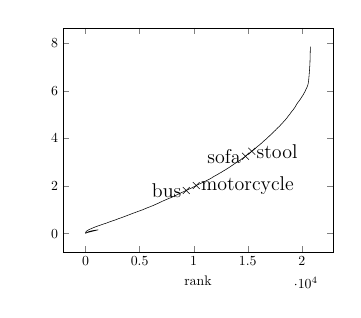
\begin{tikzpicture} [scale=0.5]
	\begin{axis} [xlabel=rank,ylabel=PMI,y label style={color=white}]
	\addplot [mark=none] coordinates {
		(0,0.00873) (295,0.08756) (590,0.12013) (885,0.14286) (1180,0.1607) (0,0.02677) (41,0.08065) (82,0.09906) (123,0.11429) (164,0.12671) (205,0.13769) (246,0.15083) (287,0.15995) (328,0.1692) (369,0.17824) (410,0.18709) (451,0.1952) (492,0.20434) (533,0.21495) (574,0.22229) (615,0.231) (656,0.23651) (697,0.24479) (738,0.25062) (779,0.25834) (820,0.26579) (861,0.27467) (902,0.28138) (943,0.28992) (984,0.29536) (1025,0.30141) (1066,0.30805) (1107,0.31515) (1148,0.3234) (1189,0.33087) (1230,0.33604) (1271,0.34317) (1312,0.34886) (1353,0.35541) (1394,0.36184) (1435,0.36848) (1476,0.37429) (1517,0.3822) (1558,0.38764) (1599,0.39293) (1640,0.40098) (1681,0.40823) (1722,0.41419) (1763,0.41853) (1804,0.42409) (1845,0.43063) (1886,0.43627) (1927,0.4425) (1968,0.44997) (2009,0.45531) (2050,0.46365) (2091,0.47124) (2132,0.47824) (2173,0.48498) (2214,0.49143) (2255,0.49638) (2296,0.50453) (2337,0.50989) (2378,0.51776) (2419,0.52444) (2460,0.53138) (2501,0.53735) (2542,0.54366) (2583,0.54887) (2624,0.55373) (2665,0.56101) (2706,0.56837) (2747,0.57471) (2788,0.58221) (2829,0.58937) (2870,0.59654) (2911,0.6041) (2952,0.61068) (2993,0.61865) (3034,0.62573) (3075,0.63437) (3116,0.64067) (3157,0.6466) (3198,0.65201) (3239,0.65797) (3280,0.6627) (3321,0.67009) (3362,0.67685) (3403,0.68503) (3444,0.69181) (3485,0.69843) (3526,0.706) (3567,0.71317) (3608,0.71995) (3649,0.72626) (3690,0.73292) (3731,0.73845) (3772,0.74578) (3813,0.75459) (3854,0.76254) (3895,0.76946) (3936,0.77635) (3977,0.78266) (4018,0.7903) (4059,0.7962) (4100,0.80308) (4141,0.81333) (4182,0.81938) (4223,0.82798) (4264,0.83336) (4305,0.83946) (4346,0.8467) (4387,0.85462) (4428,0.86113) (4469,0.86697) (4510,0.87293) (4551,0.88068) (4592,0.88904) (4633,0.89612) (4674,0.90291) (4715,0.90854) (4756,0.91565) (4797,0.923) (4838,0.92996) (4879,0.93744) (4920,0.94498) (4961,0.95142) (5002,0.95665) (5043,0.96379) (5084,0.97191) (5125,0.97696) (5166,0.98439) (5207,0.99203) (5248,0.99845) (5289,1.00495) (5330,1.01449) (5371,1.02037) (5412,1.02965) (5453,1.03662) (5494,1.04487) (5535,1.05414) (5576,1.06264) (5617,1.06717) (5658,1.07636) (5699,1.0831) (5740,1.0914) (5781,1.09796) (5822,1.10442) (5863,1.11144) (5904,1.11903) (5945,1.12612) (5986,1.13425) (6027,1.14157) (6068,1.14735) (6109,1.15481) (6150,1.16252) (6191,1.17077) (6232,1.17669) (6273,1.18503) (6314,1.19393) (6355,1.203) (6396,1.21346) (6437,1.22099) (6478,1.22696) (6519,1.2346) (6560,1.2437) (6601,1.25364) (6642,1.26292) (6683,1.26935) (6724,1.27874) (6765,1.28735) (6806,1.29474) (6847,1.30644) (6888,1.31405) (6929,1.32195) (6970,1.33023) (7011,1.33851) (7052,1.34919) (7093,1.35808) (7134,1.36713) (7175,1.3762) (7216,1.38341) (7257,1.39165) (7298,1.39816) (7339,1.40533) (7380,1.41374) (7421,1.42319) (7462,1.4328) (7503,1.43961) (7544,1.4477) (7585,1.45504) (7626,1.46103) (7667,1.4698) (7708,1.47748) (7749,1.487) (7790,1.49331) (7831,1.5012) (7872,1.50807) (7913,1.517) (7954,1.52501) (7995,1.53592) (8036,1.54448) (8077,1.55541) (8118,1.56479) (8159,1.57164) (8200,1.57983) (8241,1.58766) (8282,1.59751) (8323,1.60662) (8364,1.61387) (8405,1.62224) (8446,1.63037) (8487,1.63835) (8528,1.64723) (8569,1.658) (8610,1.66551) (8651,1.67428) (8692,1.68384) (8733,1.69278) (8774,1.70178) (8815,1.70988) (8856,1.71869) (8897,1.72736) (8938,1.73621) (8979,1.74417) (9020,1.75178) (9061,1.76248) (9102,1.76954) (9143,1.77959) (9184,1.78967) (9225,1.79854) (9266,1.80531) (9307,1.81463) (9348,1.82364) (9389,1.82984) (9430,1.83987) (9471,1.84816) (9512,1.85831) (9553,1.86775) (9594,1.87574) (9635,1.88361) (9676,1.89195) (9717,1.90189) (9758,1.90895) (9799,1.9185) (9840,1.9287) (9881,1.93976) (9922,1.94862) (9963,1.95758) (10004,1.96519) (10045,1.97336) (10086,1.98349) (10127,1.99438) (10168,2.00195) (10209,2.01153) (10250,2.02289) (10291,2.03234) (10332,2.04407) (10373,2.05289) (10414,2.06208) (10455,2.072) (10496,2.07941) (10537,2.0881) (10578,2.0964) (10619,2.10572) (10660,2.1147) (10701,2.12445) (10742,2.13346) (10783,2.14143) (10824,2.15069) (10865,2.15857) (10906,2.16899) (10947,2.17834) (10988,2.18676) (11029,2.19426) (11070,2.2011) (11111,2.20938) (11152,2.2209) (11193,2.22953) (11234,2.2379) (11275,2.24709) (11316,2.2573) (11357,2.26566) (11398,2.27685) (11439,2.28614) (11480,2.29569) (11521,2.30613) (11562,2.32011) (11603,2.32923) (11644,2.33655) (11685,2.34803) (11726,2.36436) (11767,2.3754) (11808,2.38662) (11849,2.39789) (11890,2.40615) (11931,2.41724) (11972,2.42661) (12013,2.43427) (12054,2.44468) (12095,2.45797) (12136,2.46996) (12177,2.47963) (12218,2.49114) (12259,2.49949) (12300,2.51444) (12341,2.52486) (12382,2.53655) (12423,2.54673) (12464,2.55574) (12505,2.5651) (12546,2.57442) (12587,2.58626) (12628,2.60064) (12669,2.61123) (12710,2.62377) (12751,2.63353) (12792,2.64563) (12833,2.65457) (12874,2.66541) (12915,2.67736) (12956,2.68664) (12997,2.69762) (13038,2.71349) (13079,2.72282) (13120,2.73751) (13161,2.75075) (13202,2.7607) (13243,2.76973) (13284,2.78335) (13325,2.79489) (13366,2.8062) (13407,2.81788) (13448,2.8316) (13489,2.84773) (13530,2.85953) (13571,2.86984) (13612,2.8832) (13653,2.89679) (13694,2.90957) (13735,2.92336) (13776,2.93424) (13817,2.94975) (13858,2.9605) (13899,2.97309) (13940,2.98267) (13981,2.99356) (14022,3.00853) (14063,3.01883) (14104,3.0299) (14145,3.04079) (14186,3.05526) (14227,3.06651) (14268,3.07863) (14309,3.09185) (14350,3.10502) (14391,3.1221) (14432,3.13603) (14473,3.15094) (14514,3.16297) (14555,3.17606) (14596,3.18689) (14637,3.19835) (14678,3.21075) (14719,3.22322) (14760,3.23922) (14801,3.25864) (14842,3.27703) (14883,3.28839) (14924,3.30348) (14965,3.31775) (15006,3.33425) (15047,3.34785) (15088,3.36307) (15129,3.37775) (15170,3.39287) (15211,3.4054) (15252,3.41985) (15293,3.4337) (15334,3.45112) (15375,3.46468) (15416,3.47705) (15457,3.49023) (15498,3.50164) (15539,3.52021) (15580,3.53471) (15621,3.5474) (15662,3.56152) (15703,3.57749) (15744,3.59924) (15785,3.6151) (15826,3.63472) (15867,3.65022) (15908,3.66346) (15949,3.68041) (15990,3.69407) (16031,3.70741) (16072,3.72448) (16113,3.73897) (16154,3.75398) (16195,3.77122) (16236,3.78797) (16277,3.80516) (16318,3.82257) (16359,3.84033) (16400,3.85569) (16441,3.87244) (16482,3.88989) (16523,3.90796) (16564,3.92399) (16605,3.94061) (16646,3.95372) (16687,3.96735) (16728,3.98657) (16769,4.00568) (16810,4.02217) (16851,4.04267) (16892,4.05943) (16933,4.07469) (16974,4.09078) (17015,4.11304) (17056,4.12674) (17097,4.14625) (17138,4.16004) (17179,4.17935) (17220,4.19326) (17261,4.21285) (17302,4.23273) (17343,4.24945) (17384,4.26941) (17425,4.29428) (17466,4.31052) (17507,4.32539) (17548,4.34017) (17589,4.35995) (17630,4.38333) (17671,4.40323) (17712,4.41498) (17753,4.43752) (17794,4.45723) (17835,4.4727) (17876,4.48776) (17917,4.50509) (17958,4.52632) (17999,4.54728) (18040,4.56731) (18081,4.58637) (18122,4.6068) (18163,4.62796) (18204,4.64858) (18245,4.66817) (18286,4.69012) (18327,4.71104) (18368,4.73228) (18409,4.7488) (18450,4.76772) (18491,4.79213) (18532,4.81396) (18573,4.83353) (18614,4.85713) (18655,4.88483) (18696,4.91393) (18737,4.9368) (18778,4.95964) (18819,4.98094) (18860,5.00694) (18901,5.02989) (18942,5.06233) (18983,5.08253) (19024,5.10587) (19065,5.12961) (19106,5.1567) (19147,5.17936) (19188,5.1987) (19229,5.22071) (19270,5.25074) (19311,5.27716) (19352,5.30173) (19393,5.33715) (19434,5.36873) (19475,5.40175) (19516,5.43814) (19557,5.4595) (19598,5.48969) (19639,5.51546) (19680,5.53591) (19721,5.55929) (19762,5.58441) (19803,5.61271) (19844,5.63882) (19885,5.66969) (19926,5.6969) (19967,5.72762) (20008,5.7545) (20049,5.77884) (20090,5.81302) (20131,5.83841) (20172,5.87575) (20213,5.91056) (20254,5.93799) (20295,5.97812) (20336,6.0231) (20377,6.06203) (20418,6.09435) (20459,6.13534) (20500,6.18576) (20541,6.22955) (20582,6.29717) (20623,6.421) (20664,6.62848) (20705,6.86175) (20746,7.13908) (20787,7.85674)
	};
	\addplot [mark=x,only marks,mark size = 3.5] coordinates {
		(9312,1.81529)(10235,2.01808)(14787,3.24988)(15370,3.46375)
	};
	\node [anchor=east] at (axis cs: 9312,1.81529) {\Large bus};
	\node [anchor=west] at (axis cs: 10235,2.01808) {\Large motorcycle};
	\node [anchor=east] at (axis cs: 14787,3.24988) {\Large sofa};
	\node [anchor=west] at (axis cs: 15370,3.46375) {\Large stool};
	\end{axis}
\end{tikzpicture}
\caption*{dimension: \emph{accidentally}}
\end{subfigure}
\caption{\textsc{furniture} $\Longleftrightarrow$ \textsc{vehicles}}
\end{subfigure}
\caption[The Arithmetic of Analogy]{Histograms of the top three co-occurrence dimensions satisfying the expected arithmetic of two analogies.}
\label{fig:histograms}
\end{figure}

What stands out here is the way that the analogical word-vectors tend to cluster into pairs.  This makes sense, since the formula described above indicates instances where the relationship between two of the word vectors is very similar to the relationship between the other two: this requirement is nicely satisfied by pairing word-vectors up with one another.  These dimensional values are pushed into two-dimensional projections of three-dimensional spaces in Figure~\ref{fig:inspace}, and here the well-defined parallelograms expected from this method of dimension selection become apparent.  In fact, more than just parallelograms, the shapes that begin to emerge are specifically rectangular in nature.  If we imagine extending the process of selecting dimensions where target word-vectors are clustered into pairs into higher dimensional subspaces, we can see that the vertices of the shapes that would evolve would tend towards right angles, and so this indicates an additional geometric feature of the relationships between lexical semantic representations that we might associate with analogy.

\revJB{6}{It must additionally be noted that the dimensions revealed as best suited for these analogies are not necessarily associated with co-occurrences that correspond to the conceptual basis of the analogies in any obvious way.  Returning to a point made in Chapter~\ref{sec:project}, the labels of co-occurrence dimensions associated with a given input may not reveal an immediately intuitive conceptual connection, though there will always be an opportunity for recourse to actual observations in the underlying corpus that will at least corroborate the statistical foundations of a contextualised analogy.    Furthermore, again as seen in the examples provided in Chapter~\ref{sec:project}, a more coherent profile of co-occurrence features is likely to emerge as we move into higher dimensional spaces.  Our first task is to find amongst this profile of relevant co-occurrences those dimensions which are particularly suited to completing an analogy in a prescribed way, and so the objective will be to discover, not to interpret, these analogically efficacious dimensions.  An exploration of more sophisticated techniques for selecting these dimensions will be discussed at the end of this chapter, but the application and subsequent of, for instance, machine learning techniques for learning a methodology for reliably specifying analogical subspaces will ultimately be left for the future.}

\revJB{9}{On the other hand, while we may not be able to interpret the labels associated with the dimensions of a given subspace, it may be worth consideration of the vectors inherent in the conceptual transfer implied by an analogy.  So, for instance, can we expect the vector that maps from both \emph{surgeon} to \emph{scalpel} and from \emph{butcher} to \emph{cleaver} to be in some sense a more general vector mapping from \textsc{profession} to \textsc{implement}?  If this turns out to be the case, then context specific projection based on analogical input begin to resemble the conceptual spaces of }\cite{Gardenfors2000}, \rev{with directions, oblique to the orthography of the subspace itself but consist across domains, associated with certain intensionalities.  An interesting question, then, is whether these directions can be extracted from the structure of an analogy and analysed on their own: if this conceptual vector were positioned at the origin, to which word-vector would it most closely point?  Such an analysis may be thwarted by certain factors, for instance the probable presence of negative values along some dimensions, but it still bears further analysis and should provide a direction for future work.}

Another interesting thing to note about the configurations in Figure~\ref{fig:inspace} is the oblong nature of the shapes.  In fact, it seems as though the word-vectors are orientating themselves in terms of types---though not necessarily in alignment with the conceptual categories we presumed to delineate the analogical mappings.  So, where \emph{bus} and \emph{motorcycle} might be seen as occupying a \textsc{vehicle} extent of the subspace as opposed to the \textsc{furniture} region inhabited by \emph{sofa} and \emph{stool}, \emph{surgeon} and \emph{butcher} seem to be establishing a region of \textsc{professions} while \emph{scalpel} and \emph{cleaver} could be construed in a domain of \textsc{implements}.  These distinctions are, naturally, a peculiarity of the dimensions themselves, with \emph{hands} in particular specifying a high co-occurrence with \textsc{implements}, while the preposition \emph{beneath}, with its spatial intimations, remits high values for \emph{sofa} and \emph{stool} (denotations of things that other things can be beneath); the prevalence of these same terms in co-occurrences with \emph{hearing} is less obvious but nonetheless indicative.

\begin{figure}
\centering
\begin{subfigure} [t] {0.45\textwidth}
\centering
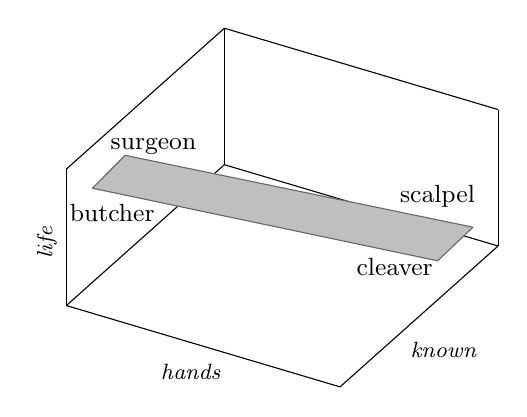
\begin{tikzpicture}
%\begin{axis}[view={120}{10},xmin=0,xmax=4.5,ymin=0,ymax=4.5,zmin=0,zmax=4.5,xlabel=gray,ylabel=relate, zlabel=tone,colormap/blackwhite]
\begin{axis}[view={120}{50},scale = 0.8,xlabel=\footnotesize\emph{known},ylabel=\footnotesize\emph{hands},zlabel=\footnotesize\emph{life},ticks=none,colormap/blackwhite]
%\addplot3 [color=black,->,ultra thick] coordinates {(0,0,0) (4,4,4)};
\addplot3[patch,patch type=rectangle,color=lightgray,fill opacity=1] coordinates {
 	(0.44529,2.40174,0.70908) (0.9647,2.54414,0.77903) (1.80307,1.13695,0.99632) (1.2979763,0.98899,0.92747)
};
\node [anchor=south] at (axis cs: 0.44529,2.2,0.70908) {\small scalpel};
\node [anchor=north] at (axis cs: 0.9647,2.3,0.77903) {\small cleaver};
\node [anchor=south] at (axis cs: 1.2979763,1.15,0.92747) {\small surgeon};
\node [anchor=north] at (axis cs: 1.80307,1.25,0.99632) {\small butcher};
%\addplot3 [color=black,->,ultra thick] coordinates {(2.2,2.2,2.2) (4,4,4)};
\end{axis}
\end{tikzpicture}
\caption{\textsc{surgery} $\Longleftrightarrow$ \textsc{butchery}}
\label{FIG:subspace}
\end{subfigure}
\hspace{0.05\textwidth}
\begin{subfigure} [t] {0.45\textwidth}
\centering
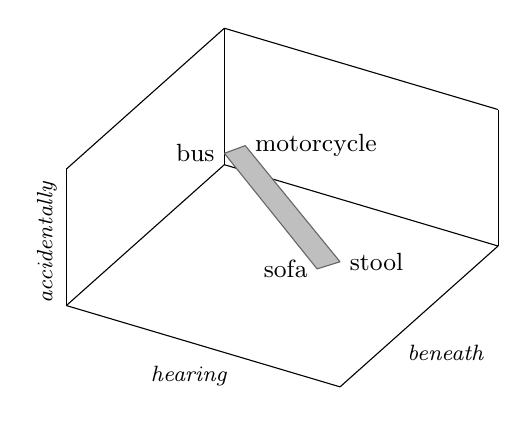
\begin{tikzpicture}
%\begin{axis}[view={120}{10},xmin=0,xmax=4.5,ymin=0,ymax=4.5,zmin=0,zmax=4.5,xlabel=gray,ylabel=relate, zlabel=tone,colormap/blackwhite]
\begin{axis}[view={120}{50},scale=0.8,xlabel=\footnotesize\emph{beneath},ylabel=\footnotesize\emph{hearing}, zlabel=\footnotesize\emph{accidentally},ticks=none, colormap/blackwhite]
%\addplot3 [color=black,->,ultra thick] coordinates {(0,0,0) (4,4,4)};
\addplot3[patch,patch type=rectangle,color=lightgray,fill opacity=1] coordinates {
 	(0.83647,1.81529,0.3181) (1.05531,2.01808,0.80923) (3.5408,3.46375,2.23614) (3.32574,3.24988,1.74923)
};
\node [anchor=east] at (axis cs: 0.83647,1.81529,0.3181) {\small bus};
\node [anchor=west] at (axis cs: 1.05531,2.01808,0.80923) {\small motorcycle};
\node [anchor=east] at (axis cs: 3.32574,3.24988,1.74923) {\small sofa};
\node [anchor=west] at (axis cs: 3.5408,3.46375,2.23614) {\small stool};
%\addplot3 [color=black,->,ultra thick] coordinates {(2.2,2.2,2.2) (4,4,4)};
\end{axis}
\end{tikzpicture}
\caption{\textsc{furniture} $\Longleftrightarrow$ \textsc{vehicles}}
\end{subfigure}
\caption[Two Analogies in Space]{The geometry of two analogies projected into subspaces defined by the three most analogically accurate dimensions.}
\label{fig:inspace}
\end{figure}

\revJB{7}{Returning objection function, there is an equivalence between the expressions $(a-b) - (c-d) = 0$ and $(a-c) - (b-d) = 0$, and so the potential impression of an inherent commitment to the idea that the conceptual relationship between $A$ and $B$ is in some sense equivalent to $A$ and $B$.  And there is an element of common sense wisdom to this: we can imagine extending the relationship between the domains of \textsc{surgery} and \textsc{butchery} to include pairings such as \emph{patient:carcass}, \emph{hospital:abattoir}, and so forth; on the other hand, we could also make an orthogonal mapping from a domain of something like \textsc{professions} to a a domain of \textsc{implements}, and expect a congruency with the vectors associated with \emph{barber:scissors}, \emph{tailor:needle}, or even \emph{writer:pen}.  This is not to say that there is comparable cohesiveness between the conceptual domains, however, and the elongated characteristic of the analogies depicted in Figure~\ref{fig:inspace} can be interpreted as indicating this imbalance.  This is in line with the psychological research of }\cite{Tversky1977}, \rev{mentioned in Chapter~\ref{sec:frames} in the context of word similarity, which notes the imbalance between comparisons between paradigmatic and peripheral concepts within or across domains.  Similarly, \cite{Ortony1979} has described the \emph{salience imbalance} inherent in many metaphors, and the implicit asymmetry of analogy that emerges from this analysis.}\footnote{\revJB{7}{It should be additionally be noted that the task of analogy completion, discussed below in Section~\ref{sec:solutions}, is likewise note necessarily symmetrical: the point $D$ implied by the question $A:B::C:X?$ might be in a considerably more dense region of a different subspace than point $C$ for $B:A::D:X?$.}}

One of the things to take away from this small-scale qualitative analysis is that, at the end of the day, any four-point analogy can be cut along at least two different conceptual axes, corresponding to the intensions that semantically bind the representations along each edge of the rectangle.  We might easily speculate that the shapes found in well-formed analogical subspaces will be elongated along the axes that correspond to what humans might tend to classify as the conceptually salient distinction inherent in the analogy, but there are presumably also a variety of ways to make an orthogonal distinction, and we can reasonably expect these secondary characteristics of the analogical relationship to emerge in higher dimensional spaces.  In fact, a reasonable hypothesis, raised in \cite{McGregorEA2016}, is that contextualised analogical planes should, as dimensionality increases, begin to assume a more sqaure shape and a more central position in a subspace.

So I think it makes sense to expand this approach to analogy modelling to cover more analogies, and to examine the way that higher dimensionalities provide a basis for geometric analysis.  In order to efficiently and systematically test the viability of context sensitive subspaces for analogy solution, I randomly select a subset of 996 analogies from the data, described above, designed by \cite{MikolovEA2013b}, and project 400 dimensional subspaces from both 2x2 and 5x5 word window base spaces using the \textsc{joint}, \textsc{indy}, and \textsc{zipped} techniques, taking, with an eye towards an analogy solving methodology, only the first three of the four words in each analogy as input.  Following this step, and as with the examples mentioned above, this experiment becomes an instance of what we might call space-fitting: in each of the six resulting subspaces (two base spaces by three dimension selection techniques), \del{I rank dimensions in order of their proximity to satisfying the equivalence relationship between legs of the analogy and then see if the analogy works out in the top $d$-dimensional projection.}\revJB{8}{I pick the top $d$ dimensions that come closest to satisfying the equation $(a-b) - (c-d) = 0$, and I then find word-vector for $X$ that, in a given $d$-dimensional subspace, is nearest to the point $x = b+c-a$.  If $X$ is $D$, then I consider the analogy to have been successfully mapped in that subspace.}

\begin{table}
\centering
\begin{tabular}{clrrrrrr}
\hline
\multicolumn{2}{l}{\emph{dimensions}} & 5 & 10 & 20 & 50 & 100 & 200 \\
\hline
\parbox[t]{2mm}{\multirow{3}{*}{\rotatebox[origin=c]{90}{ 2x2}}} & \textsc{joint} & 0.911 & 0.972 & 0.989 & 0.986 & 0.970 & 0.916 \\
& \textsc{indy} & 0.722 & 0.908 & 0.976 & 0.985 & 0.967 & 0.873 \\
& \textsc{zipped} & 0.921 & 0.975 & \revAK{4}{\emph{0.991}} & 0.987 & 0.970 & 0.919 \\
\hline
\parbox[t]{2mm}{\multirow{3}{*}{\rotatebox[origin=c]{90}{\textsc{ 5x5}}}} & \textsc{joint} & 0.941 & 0.987 & 0.996 & 0.997 & 0.995 & 0.957 \\
& \textsc{indy} & 0.697 & 0.908 & 0.973 & 0.984 & 0.962 & 0.895 \\
& \textsc{zipped} & 0.934 & 0.987 & \revAK{4}{\emph{0.999}} & 0.998 & 0.997 & 0.968 \\
\hline
\end{tabular}
\caption[Finding Spaces for Known Analogies]{Accuracy rates for solving analogies when choosing subsets of optimal dimensions from 400 dimensional subspaces picked taking the first three elements of each analogy as input.}
\label{tab:knowns}
\end{table}

Results for this experiment are reported in Table~\ref{tab:knowns}, with accuracy scores given for subspaces of 5, 10, 20, 50, 100, and 200 dimensions.  In the case of both the \textsc{joint} and \textsc{zipped} techniques, the chances of finding a satisfactory subspace are strong across the board.  This means that, on the one hand, it should be possible to pick as few as the right 5 dimensions out of a set of 400 and still find a subspace where more than 90\% of the analogies in this sampled dataset are accurately modelled, and, on the other hand, there is a way to cut the set of 400 dimensions picked without knowledge of the fourth component of an analogy in half and get likewise reliably productive geometries.  The \textsc{indy} technique doesn't do quite as well here, particularly at the lower dimensionalities where there is presumably less of a chance of finding many significant values for all the components of an analogy along co-occurrence dimensions that might have achieved high scores for a single input term independently in part by way of being infrequent and perhaps specialised.  And of course, there are quite a few ways to pick either 5 or 200 out of a set of 400, so we do not yet have an analogy solving or generating engine on our hands.

This last point leads to a further question: could there be some way, given the vast combinatory spaces of dimensional subsampling available here, to solve more or less \emph{any} version of an analogy?  If the contextualisation process is so open ended that we can geometrically constrct more or less any conceivable semantic relationship, then the first step of the contextualisation process, in which only part of the analogy is used to generate a subspace from which subsequent fully informed selection are made, doesn't really get us anything at all in the way of using three points of an analogy to find the appropriate context for discovering the fourth point.  With this in mind, I rearrange the sample of the data used to generate the results in Table~\ref{tab:knowns} such that the fourth component of each example is randomly selected from all possible fourth components across the list.  Table~\ref{tab:fakes} reports results for selecting lower dimensional subspaces expected to solve these random lexical constructs, applying the same procedure as described above for identifying optimal dimensions and then testing at various dimensionalities.

\begin{table}
\centering
\begin{tabular}{clrrrrrr}
\hline
\multicolumn{2}{l}{\emph{dimensions}} & 5 & 10 & 20 & 50 & 100 & 200 \\
\hline
\parbox[t]{2mm}{\multirow{3}{*}{\rotatebox[origin=c]{90}{2x2}}} & \textsc{joint} & 0.654 & 0.814 & 0.896 & \revAK{4}{\emph{0.930}} & 0.881 & 0.466 \\
& \textsc{indy} & 0.115 & 0.234 & 0.341 & 0.369 & 0.267 & 0.045 \\
& \textsc{zipped} & 0.616 & 0.806 & 0.892 & 0.929 & 0.887 & 0.489 \\
\hline
\parbox[t]{2mm}{\multirow{3}{*}{\rotatebox[origin=c]{90}{\textsc{5x5}}}} & \textsc{joint} & 0.657 & 0.828 & 0.901 & \revAK{4}{\emph{0.921}} & 0.835 & 0.402 \\
& \textsc{indy} & 0.129 & 0.253 & 0.338 & 0.384 & 0.277 & 0.051 \\
& \textsc{zipped} & 0.589 & 0.790 & 0.888 & 0.915 & 0.876 & 0.418 \\
\hline
\end{tabular}
\caption[Finding Spaces for Fake Analogies]{Accuracy rates for solving randomly completed analogical inputs when choosing subsets of optimal dimensions from 400 dimensional subspaces picked taking the first three elements of each lexical construct as input.}
\label{tab:fakes}
\end{table}

On the one hand, these results are impressively -- even surprisingly -- good.  It turns out, for instance, that there is some set of 50 dimensions to be selected from the 400 dimensional subspace projected by applying the \textsc{joint} technique to the inputs (\emph{Athens, Greece, Berlin}) that solves the unlikely analogy \emph{Athens:Greece :: Berlin:Impossible}.  On the other hand, though, these scores are substantially lower than those reported for established analogies in Table~\ref{tab:knowns}.  This is particularly the case for higher dimensionalities, where the options for discovering a multitude of dimensions facilitating the mapping of a randomly generated analogy evidently become confounded, and the difference is greatest of all for relatively large sets of dimensions chosen from the \textsc{indy} subspaces.  So it would seem that the overlap between independently selected co-occurrence dimensions is actually indicative of some degree of conceptual coherence after all, evidenced by the relative likelihood of solving an attested analogy versus a random one.  (It's also interesting to note that subspaces derived from smaller co-occurrence windows are more apt to yield what we might call forgiving analogical options for the randomly generated data, indicating once more that there is more conceptual association in the syntagms available in a wider co-occurrence window, as discussed in the context of relatedness versus similarity in Chapter~\ref{sec:relmeth}.)

\subsection{Searching for Solutions to Analogies} \label{sec:solutions}
Having established that there are in principle analogically productive subspaces to be discovered based on taking part of an analogy as input to a context sensitive distributional semantic model, I now explore the capacity of my methodology for completing partial analogies.  The procedure applied here is simply to take the first three terms for each analogy as input and then use an analysis of the corresponding word vectors to project subspaces following the \textsc{joint}, \textsc{indy}, and \textsc{zipped} methods.  \revJB{35}{In the proof-of-concept presented in the previous section, subspaces ranging from 5 to 200 dimensions were projected based on an evaluation of the positions of word-vectors corresponding to all four components of each analogy; these projections were made from sets of 400 dimensions selected based on an analysis of only the first three terms in each analogy, however, in order to demonstrate that there is, in principle, as way to make an informed selection from a set of dimensions that is already relatively refined.  The following experiment does away with any information about the fourth component of each analogy.}  These spaces then become the basis for a geometric solution to the analogy, taking the fourth point to be the word-vector that most closely completes the parallelogram indicated by the three input vectors.  Unlike with the experiments on relatedness, similarity, metaphor, and coercion described in the previous two chapters, this experiment is completely unsupervised; the hypothesis tested is that contextualisation alone should provide a basis for the geometric modelling of the conceptual alignments inherent in analogy.

\begin{table}
\centering
\begin{tabular}{clrrrrrrr}
\hline
\multicolumn{2}{l}{\emph{dimensions}} & 5 & 10 & 20 & 50 & 100 & 200 & 400 \\
\hline
\parbox[t]{2mm}{\multirow{6}{*}{\rotatebox[origin=c]{90}{2x2}}} & \textsc{joint} & 0.020 & 0.052 & 0.082 & 0.164 & 0.221 & 0.271 & 0.274 \\
& \textsc{indy} & 0.010 & 0.079 & 0.163 & 0.315 & 0.406 & 0.450 & 0.469 \\
& \textsc{zipped} & 0.016 & 0.055 & 0.128 & 0.234 & 0.280 & 0.294 & 0.282 \\
& \textsc{CBoW} & - & - & 0.180 & 0.435 & - & 0.588 & 0.612 \\
& \textsc{SG} & - & - & 0.191 & 0.394 & - & 0.630 & \revAK{4}{\emph{0.674}} \\
& \textsc{SVD} & - & - & 0.035 & 0.033 & - & 0.025 & 0.026 \\
\hline
\parbox[t]{2mm}{\multirow{6}{*}{\rotatebox[origin=c]{90}{\textsc{5x5}}}} & \textsc{joint} & 0.016 & 0.048 & 0.094 & 0.199 & 0.291 & 0.326 & 0.327 \\
& \textsc{indy} & 0.017 & 0.077 & 0.182 & 0.340 & 0.438 & 0.511 & 0.509 \\
& \textsc{zipped} & 0.016 & 0.058 & 0.150 & 0.307 & 0.357 & 0.378 & 0.367 \\
& \textsc{CBoW} & - & - & 0.200 & 0.448 & - & 0.607 & 0.632 \\
& \textsc{SG} & - & - & 0.175 & 0.397 & - & 0.622 & \revAK{4}{\emph{0.672}} \\
& \textsc{SVD} & - & - & 0.043 & 0.045 & - & 0.047 & 0.051 \\
\hline
\end{tabular}
\caption[Solving Analogies]{Accuracy rates for analogy solution by various techniques with various parameters, taking the first three words in an analogy as input and then providing the fourth word as output.}
\label{tab:solutions}
\end{table}

Results for my methodologies as well as the \texttt{word2vec} modelling techniques and static SVD models, with various parametric specifications, are reported in Table~\ref{tab:solutions}.  With the exception of the most low dimensional subspaces, the \textsc{indy} technique performs the best of the context sensitive methodologies, eventually offering the expected solution to more than half of the analogies in the dataset for higher dimensional subspaces (and the difference here with the next best \textsc{zipped} results is approaching significance with $p = .028$ based on a permutation test).  This is an interesting result in the context of the lower \textsc{indy} scores in Tables~\ref{tab:knowns} and \ref{tab:fakes} above: taken altogether, this suggests that this technique returns sparser subspaces consisting of more specialised co-occurrence dimensions salient to only one of the inputs, which make it harder to consistently find dimensions where the analogical relationships play out in the desired way, given full knowledge of the conceptual relationships being mapped, but by the same token less likely to find dimensions that complete an arbitrary construct, as well.  So on balance, co-occurrence dimensions that are more likely to be have a few strong values for a small set of relevant words would seem to correspond to the kind of contextualised conceptual specificity that lends itself to the productive generation of analogical completions.

The context sensitive approaches exhibit steadily improving performance up to 200 dimensions, but then seem to level off after this point, suggesting once again that, in the case of count-based distributional models, a sufficient but still, relative to the dimensionality of the base spaces, small number of highly relevant co-occurrence dimensions are best suited for extrapolating conceptual geometry.  Also of note is the improvement across the board moving from lower to higher sized co-occurrence windows.  So it would seem that in the case of the semantic alignments at play in analogy, the syntagmatic information available across wider portions of sentences gives more of a semantic handle to the resulting geometric relationships of word-vectors.  Finally, and not dissimilarly to results for previous experiments, there is not too much to pick between the \textsc{joint} and \textsc{zipped} techniques, though the latter does, particularly in lower dimensionalities where it exhibits some of the specificity afforded by the \textsc{indy} method, offer marginally better outcomes.

In terms of the static semantic models, the SVD approach completely collapses on this test.  It would seem that the move of dimension-wise normalisation of the abstracted matrix of optimally informational vectors, which proved so effective for word relatedness modelling and at least adequate on other tests, knocks the lexical representations of the model out of the neat geometric relationships that are sought here.  The \texttt{word2vec} techniques, on the other hand, are outstanding, with any marginal differences in performance between what is reported here and results reported in the original literature as discussed above presumably attributable to variations in the underlying corpora involved in training the models (and the probability of the difference between the top 2x2 window, 400 dimensional skip-gram model and the 5x5 window, 200 dimensional \textsc{indy} subspaces being attributable to variations in the data is $p = .018$).  The skip-gram technique, which \cite{MikolovEA2013} conjectured should be particularly good at handling what they termed as semantic (meaning more overtly intensional) analogies, does consistently better than the CBoW technique at higher dimensionalities, though, interestingly, not at lower dimensionalities, indicating that the co-occurrence predicting approach gains in semantic potency as more informational leeway is allowed into the model.

\begin{figure}
\centering
\small
\begin{subfigure}{1 \textwidth}
\begin{tikzpicture}
  \begin{axis}[width=1*\textwidth,xtick=data,ybar=2*\pgflinewidth,symbolic x coords={countries,currencies,states,demonyms,families,antonyms},enlarge x limits=0.25,ymin=0,height=0.2\textheight,ylabel={accuracy},major x tick style=transparent,legend cell align=left,enlarge x limits = {abs=1cm},ymax=1]
    \addplot[fill=gray,opacity=0.2] coordinates {(countries,0.698) (currencies,0.167) (states,0.474) (demonyms,0.886) (families,0.909) (antonyms,0.273)};
    \addplot[fill=gray,opacity=0.4] coordinates {(countries,0.866) (currencies,0.133) (states,0.533) (demonyms,0.898) (families,0.818) (antonyms,0.273)};
    \addplot[fill=gray,opacity=0.6] coordinates {(countries,0.453) (currencies,0.000) (states,0.395) (demonyms,0.739) (families,0.545) (antonyms,0.068)};
    \addplot[fill=gray,opacity=0.8] coordinates {(countries,0.819) (currencies,0.000) (states,0.533) (demonyms,0.761) (families,0.545) (antonyms,0.159)};
    \legend{\textsc{CBoW},\textsc{SG},\textsc{zipped},\textsc{indy}}
  \end{axis}
\end{tikzpicture}
\end{subfigure}
\begin{subfigure}{1 \textwidth}
\begin{tikzpicture}
  \begin{axis}[width=1*\textwidth,xtick=data,ybar=2*\pgflinewidth,symbolic x coords={adverbs,comparatives,gerunds,tenses,plurals,conjugates},enlarge x limits=0.25,ymin=0,height=0.2\textheight,ylabel={accuracy},major x tick style=transparent,legend cell align=left,enlarge x limits = {abs=1cm},ymax=1]
    \addplot[fill=gray,opacity=0.2] coordinates {(adverbs,0.200) (comparatives,0.549) (gerunds,0.661) (tenses,0.754) (plurals,0.650) (conjugates,0.719)};
    \addplot[fill=gray,opacity=0.4] coordinates {(adverbs,0.200) (comparatives,0.434) (gerunds,0.661) (tenses,0.551) (plurals,0.700) (conjugates,0.579)};
    \addplot[fill=gray,opacity=0.6] coordinates {(adverbs,0.020) (comparatives,0.265) (gerunds,0.492) (tenses,0.261) (plurals,0.562) (conjugates,0.140)};
    \addplot[fill=gray,opacity=0.8] coordinates {(adverbs,0.040) (comparatives,0.230) (gerunds,0.424) (tenses,0.261) (plurals,0.812) (conjugates,0.298)};
%    \legend{\textsc{CBoW},\textsc{SG},\textsc{indy}}
  \end{axis}
\end{tikzpicture}
\end{subfigure}
\caption[Comparative Analogy Completion Scores] {Accuracy rates for various modelling techniques on semantically delineated subsets of the data, for 5x5 word window, 200 dimensional spaces.}
\label{fig:anaparisons}
\end{figure}

In order to tease out the operations of various methodologies a bit more, I separate the data into 12 different conceptual categories, in line with the divisions provided by the original data, though I will not dwell at this point on the theoretical issues raised by the distinctions initially made between semantics and syntax.  The categories split out as follows, including the numbers of instances of each category in the sampled data:

\begin{itemize}[noitemsep]
\item[] 232 countries and capitals (\emph{Germany:Berlin :: Iran:Tehran});
\item[] 30 countries and currencies (\emph{Mexico:peso :: India:rupee});
\item[] 152 American states and cities (\emph{Cincinnati:Ohio :: Memphis:Tennessee});
\item[] 22 countries and demonyms (\emph{Denmark:Danish :: China:Chinese});
\item[] 50 familial relationships (\emph{father:mother :: son:daughter});
\item[] 44 antonyms (\emph{logical:illogical :: informative:uninformative});
\item[] 113 adjectives and adverbs (\emph{swift:swiftly :: furious:furously});
\item[] 59 adjectives and their comparative and superlative forms (\emph{good:better :: tough:tougher});
\item[] 88 verbs and gerunds (\emph{go:going :: write:writing});
\item[] 69 present participles and past tense verbs (\emph{screaming:screamed :: saying:said});
\item[] 80 singular and plural nouns (\emph{woman:women :: pineapple:pineapples});
\item[] 57 singular and plural verb conjugations (\emph{think:thinks :: say:says}).
\end{itemize}

\noindent Figure~\ref{fig:anaparisons} illustrates the accuracy scores for these subsets of the data for four different semantic modelling techniques: the two \texttt{word2vec} methods and my \textsc{zipped} and \textsc{indy} methods, all with parameters set to 5x5 word windows and 200 dimensions, presented as a bar chart for the sake of visual comparison within and across categories.  The context sensitive methodologies, represented by the darker bars to the right in each categorical cluster, perform somewhat comparably with the neural network models in the cases of conceptual domains such as demonyms and plurals, with the \textsc{indy} method in particular outperforming all other methods for mapping the expected relationships between singular and plural nouns (though the difference is only marginally significant, with $p = .031$ on a permutation test between the \textsc{indy} results, with accurracy of 0.812, and the skip-gram results of 0.700).  The \textsc{indy} technique also does a good job of mapping pairs of countries and capital cities, again with no statistical significance between the \textsc{indy} score of 0.819 and the skip-gram score of 0.866 (p = .150), though the \textsc{zipped} technique does fall down here, with an accuracy of just 0.453.  The overall impression here is that the contextual methodologies seem to do particularly well in instances where there is an expectation of close co-occurrence relationships along one axis of the analogical construct: so, singular and plural forms of nouns are likely to have similar co-occurrence profiles, particularly under the broader 5x5 word window tabulating parameter, and likewise with the names of countries and the gentilics of their inhabitants.

Where context sensitive projections do less well is on the analogies involving shifts that relate to the more abstract conceptual domains of grammatical classes, such as the comparison of adjectival and adverbial forms or the mappings between antonyms.  And it is interesting to note that these approaches fail to complete even a single instance of mapping from country name to national currency.  One theory here is that the dimensions of currency word-vectors are too sparse and obscure to develop into a coherent conceptual region within subspaces constrained by co-occurrences primarily relating to country names, a hypothesis supported anecdotally by instances of failed analogies such as \emph{Denmark:krone :: Angola:Angolan} and \emph{Japan:yen :: Argentina:Argentine}---indeed, in most cases, inputs involving one currency and two country names seem to map to the demonym rather than to the currency of the unpaired country.  A sense emerges that these subspaces match the expected patterns in the dataset best when there is recourse, by way of co-occurrence tendencies, to distinct regions in the contextualised conceptual space of lower dimensional projections.  In fact, on the whole, all the methods examined here seemed to do better on tests involving conceptual domains which we might qualitatively describe as consisting of more distinctly defined regions, with the looser semantics of comparisons between adjectives and adverbs or pairs of antonyms tending to foil the models.  For instance, while there is a clear semantic relationship to be drawn between words such as \emph{happy} and \emph{unhappy} or, orthogonally, \emph{unhappy} and \emph{unimpressed} when they are extracted from their natural sentential habitat, there is in fact quite a bit of semantic distinction in how these words are actually used, and presumably a corresponding disparity in co-occurrence profile.  This insight will be revisited below in Section~\ref{sec:datanote}.

Finally, in order to analyse the performance of the \textsc{indy} technique in terms of statistical features of co-occurrences rather than suppositional conceptual categories, Figure~\ref{fig:xando} presents hits and misses in the 200 dimensional, 5x5 word window subspaces as functions of the number of non-zero valued co-occurrence dimensions jointly shared by all three input word-vectors versus the sum of independent non-zero valued dimensions for each word-vector.  The trend that emerges here is a distinct clustering of hits for subspaces picked by words that have an overall lower number of positive co-occurrence dimensions, and then secondarily for subspaces invoked by words with a relatively high overlapping co-occurrence profile compared to their independent distributions of co-occurrences.  In the first instance, this would seem to indicate that more specialised relationships, denoted by words that either simply come up less or else come up in more particular sentential contexts, are more prone to picking the subspaces where a fourth component of an analogy will be successfully identified.  In the second instance, solutions to analogies involving words that have a relatively significant degree of overlap in terms of the way that they tend to be used emerge.  In both cases, it makes sense that the \textsc{indy} technique, which will hone in on specialised co-occurrences, should provide a good basis for contextualising partial analogies.

\begin{figure}
\centering
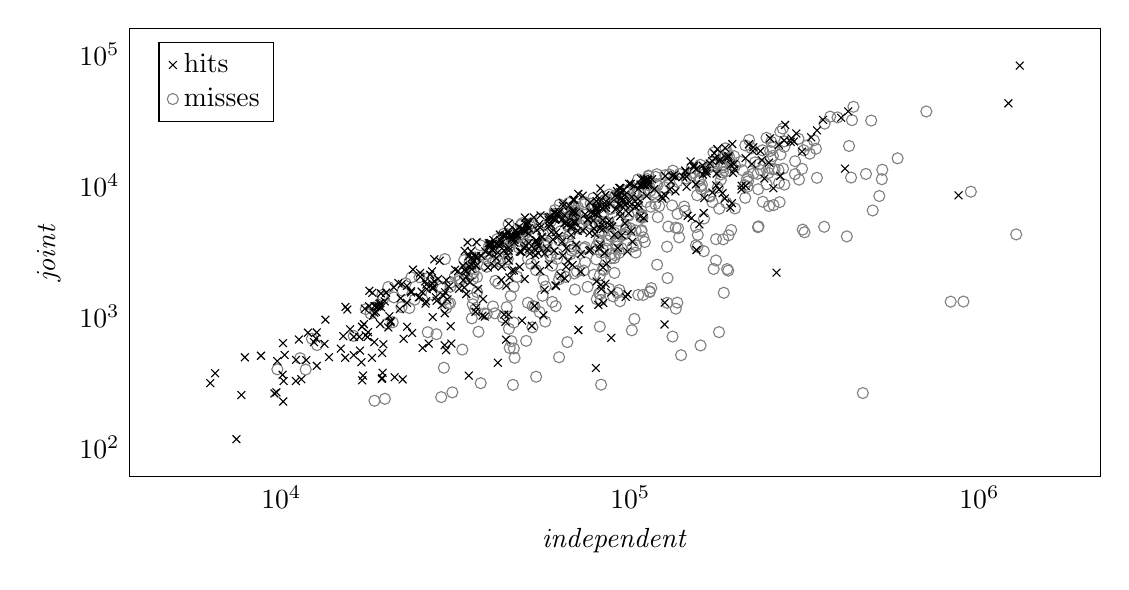
\begin{tikzpicture}
\begin{axis}[scatter/classes={x={mark=x,draw=black},o={mark=o,draw=gray}},xmode=log,ymode=log,x post scale = 1.8,ylabel=\emph{joint},xlabel=\emph{independent},tick style={draw=none},legend pos=north west,legend cell align = {left}]
\addplot[scatter,only marks,scatter src=explicit symbolic]
table[meta=label] {
x y label
151038 12468 o
38554 2768 o
188470 7353 o
68555 5931 o
117934 8242 o
129409 10502 o
22706 1783 o
43783 2597 o
22100 1173 o
90377 8310 o
24869 1983 o
29417 2731 o
71578 4989 o
34608 2582 o
16113 707 o
85683 7796 o
9738 393 o
102674 953 o
45235 3490 o
30542 1681 o
18009 1048 o
100965 781 o
184442 3865 o
179470 756 o
17457 1133 o
65990 634 o
45402 1431 o
11740 391 o
20244 1672 o
94896 7790 o
19452 1448 o
28536 1685 o
11317 478 o
26258 755 o
35151 2097 o
89916 2780 o
155711 3389 o
43856 3723 o
33402 2685 o
12653 602 o
104454 7105 o
22259 1566 o
57007 910 o
46326 895 o
53691 345 o
144662 11273 o
27818 729 o
52494 1197 o
35129 963 o
38765 1042 o
93363 1301 o
91228 3823 o
131687 7020 o
97364 4801 o
37247 308 o
45628 645 o
92056 3804 o
83449 3217 o
265592 13094 o
46584 481 o
29219 404 o
46356 567 o
44870 801 o
52407 822 o
36701 761 o
50844 1266 o
46074 299 o
82427 300 o
30893 262 o
80004 4992 o
83664 6014 o
87029 6646 o
112684 11868 o
85114 5206 o
81360 3814 o
78629 2074 o
83212 6246 o
61572 3007 o
51879 5124 o
69771 5522 o
78239 7977 o
48195 4176 o
62710 7126 o
82569 5002 o
91793 3416 o
52024 3505 o
54537 3525 o
66710 7339 o
51467 4624 o
41835 1777 o
60757 6464 o
60698 6043 o
36406 1526 o
43206 3349 o
81383 1494 o
83363 2296 o
88072 2772 o
40559 2623 o
28856 1628 o
44792 5074 o
43382 4256 o
39348 3426 o
98895 5859 o
73744 7165 o
63094 2070 o
67866 3186 o
67306 2978 o
81791 2058 o
77392 6768 o
73133 5174 o
80098 1350 o
35748 2805 o
81886 1475 o
83836 2253 o
56358 1894 o
54938 1076 o
68620 6896 o
90036 2141 o
39218 2671 o
71510 4685 o
67649 3406 o
105357 8838 o
109970 3688 o
42335 2598 o
59729 1286 o
57883 3200 o
74159 3377 o
42267 2754 o
50288 648 o
37142 3485 o
87692 6586 o
107693 5785 o
90652 3588 o
73420 2232 o
64254 3919 o
96213 4212 o
104003 3475 o
92739 3040 o
101485 3400 o
50880 2749 o
90181 2930 o
70668 6207 o
67305 5919 o
187408 19172 o
238873 18503 o
827349 1292 o
900086 1294 o
136313 1270 o
53187 1183 o
1274906 4218 o
234566 14549 o
945059 8932 o
108690 1452 o
53631 2248 o
111813 11160 o
112859 11724 o
24087 1338 o
119270 2476 o
33932 2034 o
40886 1052 o
81101 5369 o
59181 2877 o
38090 2488 o
186957 17184 o
26904 1470 o
428892 11460 o
489818 31238 o
417013 4071 o
65993 6645 o
55364 5566 o
90097 8115 o
105205 11103 o
150100 13609 o
94436 8125 o
173443 14122 o
64584 6036 o
49838 4266 o
171755 7442 o
162524 5572 o
154128 4807 o
473164 12210 o
114180 9081 o
129288 12089 o
103532 4518 o
118847 10193 o
44403 3875 o
102938 9011 o
110492 10653 o
41545 3879 o
32431 1868 o
49226 4601 o
56308 4210 o
51939 2513 o
67769 6174 o
69113 3261 o
68207 6691 o
67284 5845 o
40133 3296 o
359169 4822 o
136452 6049 o
160410 10082 o
81358 4447 o
59204 5323 o
159526 9370 o
79832 2716 o
107640 4546 o
47867 4049 o
43116 979 o
127562 1266 o
494551 6424 o
107799 5982 o
29670 1154 o
89221 1417 o
127775 1956 o
114771 1640 o
113680 1548 o
173207 2294 o
113541 1530 o
70287 2193 o
30517 1802 o
463505 259 o
28703 241 o
19797 234 o
18481 226 o
526934 13146 o
525346 11131 o
516712 8283 o
109614 9171 o
181927 12100 o
87927 2991 o
20081 878 o
206965 15142 o
120962 6949 o
171801 15041 o
82397 1331 o
29445 1343 o
20844 899 o
56423 3567 o
310420 13363 o
191148 4151 o
108885 4005 o
82440 3055 o
134806 4747 o
232851 4857 o
50200 3553 o
231194 12233 o
84388 7715 o
209581 13032 o
255846 19441 o
216377 9755 o
232352 9337 o
321278 20193 o
296172 12174 o
248513 13591 o
373695 33467 o
175891 2666 o
360118 29570 o
245526 23049 o
218781 22222 o
392254 32997 o
57527 3614 o
89805 4367 o
59648 2436 o
583110 16080 o
213273 8021 o
313753 18515 o
704713 36643 o
69072 2120 o
190772 2230 o
199733 14096 o
99986 4688 o
38765 2386 o
194448 4560 o
47893 3352 o
142591 6884 o
217350 10720 o
217601 11637 o
273872 13404 o
158662 12690 o
97816 9150 o
167742 13639 o
182763 14312 o
157092 10811 o
58910 2899 o
75392 1677 o
69349 1598 o
35420 1375 o
74204 2579 o
435582 39796 o
296448 15278 o
227529 14970 o
215616 11187 o
225223 12303 o
431474 31452 o
276192 10124 o
212807 10025 o
107454 4460 o
258993 13310 o
254989 13250 o
139718 504 o
62460 486 o
335583 22047 o
62460 1913 o
189339 2290 o
134924 1142 o
85919 3785 o
97310 4346 o
87928 4082 o
155978 4182 o
57158 1684 o
249610 6941 o
342364 11406 o
185200 1510 o
38148 1049 o
61110 1194 o
181634 11026 o
158777 9786 o
87027 4227 o
128361 4845 o
40390 1188 o
154053 3475 o
158896 598 o
252764 15906 o
269311 17165 o
326581 17434 o
96941 4606 o
48528 4971 o
36366 1993 o
35360 1920 o
95711 7749 o
176708 14629 o
132341 12940 o
66107 5010 o
175965 3877 o
179745 6628 o
48966 5133 o
222020 19202 o
21011 1392 o
30669 1813 o
107461 5918 o
155354 8394 o
257157 7057 o
266600 10429 o
26329 1961 o
44531 2729 o
125909 11946 o
117396 8794 o
148643 11517 o
73537 3294 o
12235 673 o
105733 8787 o
74222 7407 o
125085 9666 o
95014 4177 o
66332 3750 o
114419 6860 o
86869 1623 o
161849 12855 o
167418 13791 o
86978 5140 o
56025 1433 o
35859 1125 o
74833 5386 o
51384 5024 o
69415 6359 o
213423 20181 o
251463 18303 o
236344 13050 o
253266 21482 o
107320 5685 o
46075 3813 o
92275 5362 o
102115 8770 o
65292 1999 o
34974 2798 o
185938 16187 o
138402 12179 o
190285 17428 o
163919 13328 o
79020 6933 o
63158 4462 o
199339 6657 o
119646 9982 o
65148 5609 o
48250 3757 o
81498 3607 o
102502 8623 o
69561 6194 o
256165 16759 o
239458 7485 o
38967 2995 o
58297 4458 o
69255 5370 o
66252 4853 o
76948 7250 o
119017 12155 o
231968 4787 o
83043 4406 o
80042 3452 o
315376 4378 o
108223 5659 o
187464 12773 o
267634 7434 o
303094 22670 o
30443 1259 o
93028 1585 o
137937 4000 o
184101 12572 o
35330 1234 o
30103 1245 o
98754 5965 o
70030 5738 o
98219 8797 o
103552 3063 o
23569 1981 o
61609 2739 o
132139 9513 o
119779 5714 o
87027 8501 o
78202 6912 o
127372 3397 o
41033 1866 o
94328 3302 o
311651 4586 o
136013 10665 o
191214 15568 o
31448 2041 o
19616 1371 o
84537 7651 o
57220 3477 o
70722 6810 o
273243 27139 o
69191 2638 o
84830 7226 o
91239 7233 o
169153 8214 o
46316 1679 o
85275 3276 o
118153 11605 o
81735 833 o
276086 19687 o
44225 1174 o
132057 699 o
76930 5113 o
35586 2170 o
162368 3139 o
49091 4015 o
56707 3449 o
117898 7179 o
51862 4796 o
158560 11306 o
44022 3936 o
143303 6393 o
185109 13724 o
177936 9615 o
136997 4694 o
62570 3802 o
67044 4227 o
96320 6260 o
248804 12436 o
276045 21633 o
245552 10184 o
268823 25697 o
192434 16197 o
198252 16687 o
158540 14336 o
173014 17827 o
32261 1928 o
77450 5023 o
182061 13611 o
168612 8353 o
33000 556 o
45094 572 o
51348 3501 o
47391 2005 o
79002 5819 o
304192 11049 o
112867 10010 o
91786 1509 o
105369 1455 o
23259 1155 o
18471 1167 o
92265 8585 o
423110 19969 o
111071 7464 o
340073 19031 o
90377 8310 x
41379 3573 x
48751 4671 x
40212 3563 x
50319 4448 x
93474 6308 x
50137 3459 x
53724 3810 x
78678 4658 x
84331 3042 x
42175 3457 x
42767 3607 x
40068 3228 x
86868 5362 x
49665 3310 x
98785 6116 x
157707 5041 x
19438 523 x
25983 1301 x
28106 1923 x
22901 1704 x
18461 634 x
28415 2655 x
38271 993 x
42660 1886 x
48188 3122 x
6461 367 x
6255 308 x
17242 869 x
19184 872 x
12623 752 x
17025 831 x
27841 1313 x
59228 5012 x
34437 352 x
11405 330 x
42371 3819 x
43700 4136 x
39632 3509 x
34519 2412 x
41378 3562 x
12631 418 x
88705 4845 x
79659 402 x
34356 2868 x
36238 3676 x
44741 4287 x
35186 2813 x
30560 838 x
19403 332 x
21109 342 x
7434 115 x
22262 329 x
9677 262 x
17041 324 x
19440 337 x
16134 695 x
25001 2000 x
17840 1191 x
41701 441 x
37386 2891 x
30696 618 x
49381 4592 x
41694 3063 x
39047 2355 x
54847 5063 x
68324 6371 x
64750 5923 x
25809 1843 x
19507 370 x
19604 611 x
22400 672 x
13292 615 x
17865 1565 x
51094 4277 x
29469 1521 x
29135 1436 x
15455 1126 x
18224 1510 x
70946 783 x
71356 1130 x
17675 694 x
10105 623 x
8742 499 x
7680 250 x
19101 1245 x
17719 756 x
18767 1186 x
14799 565 x
26096 1611 x
38405 3125 x
33883 2009 x
36321 2772 x
35991 1082 x
36207 1166 x
33189 1885 x
15737 795 x
19765 1299 x
23538 1517 x
21854 1134 x
48170 2380 x
45719 3844 x
9728 454 x
29375 1054 x
11917 748 x
12567 674 x
33424 1657 x
7859 485 x
10152 320 x
29644 551 x
24935 1402 x
19219 1266 x
29913 1342 x
10218 506 x
13372 941 x
44026 662 x
60344 5520 x
10078 357 x
16117 504 x
15260 1179 x
18498 1195 x
80018 1845 x
26024 1748 x
16800 546 x
23815 2271 x
23514 1555 x
27447 1851 x
45733 2225 x
18183 481 x
11012 464 x
26429 618 x
11007 320 x
10121 223 x
13693 487 x
46430 2237 x
48704 3103 x
11781 462 x
154695 3205 x
176627 12278 x
37828 1353 x
22146 1762 x
20973 1664 x
44111 1709 x
44794 3169 x
96962 1404 x
46546 3841 x
19287 1493 x
33533 2270 x
35511 2669 x
52207 844 x
56764 3006 x
15039 705 x
30201 1685 x
32090 2216 x
28838 1219 x
21636 1792 x
19005 1192 x
18472 1063 x
16959 445 x
19960 1514 x
43874 908 x
20388 999 x
41248 2776 x
45716 3956 x
17444 714 x
18661 1081 x
18285 1008 x
88147 684 x
103301 6850 x
24966 2138 x
15240 482 x
17139 352 x
65788 4991 x
19338 1168 x
25877 1249 x
20563 923 x
20554 900 x
20252 821 x
55097 2213 x
53164 1199 x
61321 4366 x
11222 664 x
9554 257 x
36179 2435 x
27005 2199 x
26696 2075 x
27142 985 x
46885 4133 x
34943 3134 x
39712 3632 x
90581 6569 x
92449 7167 x
68588 7752 x
58303 4842 x
54487 3025 x
100208 10261 x
63715 3706 x
67596 4724 x
55281 5888 x
64132 6965 x
50744 5020 x
66822 7001 x
68636 5263 x
69467 5278 x
76521 7356 x
64080 7337 x
50325 4968 x
82677 5018 x
105399 9405 x
111399 10756 x
72991 8333 x
55177 4744 x
60561 6086 x
70948 8595 x
46508 3640 x
51537 3016 x
36590 1614 x
100525 4472 x
53953 4555 x
69156 5145 x
34157 3662 x
33529 3159 x
39305 3614 x
33754 2190 x
111296 8285 x
96467 5127 x
104744 7243 x
82052 9457 x
60740 6268 x
42804 2390 x
66243 2639 x
97994 3123 x
35880 2836 x
42204 3585 x
82345 1735 x
29702 1880 x
39437 3462 x
40339 3202 x
44585 4421 x
52854 5685 x
70594 4489 x
64894 1943 x
85222 7528 x
81351 3296 x
72143 2983 x
69140 7741 x
65429 2385 x
33867 1478 x
101379 3707 x
92066 3315 x
84868 1773 x
35088 2285 x
39466 3003 x
51135 3623 x
36165 2426 x
53735 3755 x
81821 3526 x
94406 4159 x
89866 4175 x
98114 1472 x
83666 1263 x
59981 3850 x
61013 1718 x
63153 2047 x
68322 2462 x
85479 2514 x
64029 2909 x
58389 2475 x
69823 6170 x
58454 5120 x
61331 5504 x
421005 36705 x
256780 9503 x
179499 9284 x
871357 8383 x
1210797 42274 x
1305007 82136 x
22930 831 x
161001 14142 x
171651 15295 x
235824 18252 x
401774 32827 x
179637 15459 x
93525 9540 x
59351 4395 x
87178 4944 x
43479 1031 x
54264 3590 x
105162 7887 x
44513 2911 x
122882 8202 x
40754 2414 x
54500 3421 x
49738 4450 x
83452 4628 x
92988 9548 x
277640 28967 x
224983 19528 x
134620 8986 x
105770 7019 x
329675 23247 x
83437 2358 x
356383 31570 x
266359 20374 x
53421 2455 x
289402 22826 x
162223 6140 x
75512 5517 x
99730 6946 x
186441 7927 x
342637 26283 x
67713 4181 x
53357 2935 x
78573 6138 x
61214 1702 x
298836 24885 x
310186 18089 x
72055 2187 x
99405 7448 x
131983 11783 x
49727 4537 x
83307 5403 x
96393 8462 x
60809 5475 x
111964 10954 x
197947 14510 x
183730 8709 x
218697 20596 x
79459 6036 x
152016 13738 x
85122 6742 x
195945 20660 x
268875 11763 x
213880 9881 x
177458 18927 x
44886 3343 x
21975 1372 x
57598 3300 x
35143 2455 x
69922 3508 x
48909 925 x
56787 1593 x
186916 19284 x
165266 12315 x
37686 1011 x
56337 1015 x
44744 1029 x
80512 6811 x
80505 6611 x
93620 8886 x
62166 6070 x
27428 2724 x
49881 5671 x
59043 5752 x
61238 5984 x
79889 6441 x
45192 4098 x
68296 6077 x
106754 5800 x
44787 5088 x
47904 4783 x
80691 6133 x
50734 5256 x
102722 9881 x
249482 14901 x
242045 11264 x
237971 15550 x
40529 3818 x
224322 18272 x
198513 13271 x
117160 9350 x
85211 7117 x
181373 15677 x
165422 12870 x
161439 12055 x
163634 12982 x
154048 10163 x
133586 12077 x
79810 6635 x
111954 11141 x
55766 4007 x
76392 4329 x
93506 5797 x
27054 1778 x
83032 6688 x
83149 6679 x
78343 5385 x
42256 4206 x
74173 5998 x
112262 10114 x
65564 5245 x
27714 1397 x
88197 1519 x
22901 1266 x
129678 9297 x
143840 12763 x
175193 16052 x
110096 10017 x
125942 11798 x
94098 7043 x
115376 11127 x
109166 11133 x
130737 10711 x
76961 6213 x
109105 10030 x
79900 6747 x
58467 5428 x
62540 6247 x
81858 7540 x
91512 9031 x
79148 4254 x
81911 4676 x
208020 9292 x
75472 5435 x
68721 6233 x
144872 9750 x
125998 8346 x
62344 4110 x
73087 4524 x
293941 21602 x
82562 1613 x
168767 14671 x
84801 8421 x
60563 3158 x
141475 11631 x
106841 9965 x
76147 3155 x
154401 13311 x
112474 10927 x
67852 4879 x
33155 2431 x
196891 12433 x
213802 16134 x
144909 11651 x
53504 3192 x
80310 8294 x
208300 9923 x
46010 4143 x
47367 4250 x
55871 4041 x
99173 10292 x
143609 12963 x
58267 5710 x
162744 7986 x
51204 4690 x
47408 4132 x
32293 1622 x
25230 1540 x
17339 1140 x
107034 10143 x
65517 3316 x
123606 7903 x
96604 7117 x
222960 14541 x
151993 14184 x
107387 11213 x
43151 4140 x
46972 4534 x
46999 4462 x
145952 5846 x
64708 5120 x
36140 2888 x
51207 3257 x
251238 22863 x
95833 9170 x
87413 7205 x
92054 8207 x
110327 10915 x
79970 7563 x
95015 7704 x
110109 10136 x
193995 14352 x
94478 8064 x
12404 634 x
125257 865 x
23691 745 x
288118 21463 x
275933 22008 x
25389 572 x
29362 600 x
31469 2264 x
149786 5629 x
27151 1627 x
27193 1668 x
125469 1269 x
80949 1220 x
16721 696 x
109297 5621 x
195372 7307 x
193416 6745 x
44023 4147 x
176283 9978 x
171783 8820 x
43418 3173 x
34724 1825 x
44811 2665 x
190647 16348 x
134557 11528 x
76798 3212 x
173885 17566 x
187879 16266 x
100980 8134 x
45053 1975 x
49790 1922 x
262195 2154 x
24734 1392 x
63616 5482 x
411952 13407 x
191096 16746 x
148748 15207 x
};
\legend{hits,misses}
\end{axis}
\end{tikzpicture}
\caption[Analogical Hits and Misses]{A scatter plot of hits and misses for analogy solution as functions of the number of jointly non-zero dimensions versus independently non-zero dimensions, with both axes scaled logarithmically.}
\label{fig:xando}
\end{figure}

So it looks like what's happening is that, as the overlap between the words involved in an analogy decreases, the expected location of the fourth point is pushed into problematic regions of the space on a dimension-by-dimension basis.  This can be visualised by once again considering the dimensional analysis of analogy illustrated in Figure~\ref{fig:histograms}.  In the case where the dimension-selecting word is the first component of the analogy (\emph{A} in \emph{A:B::C:D}), the expected location of the fourth point is actually pushed into the negative region of the dimension, where there is no information to be found.  In cases where \emph{B} or \emph{C} are the selecting words, \emph{D} would be expected to be paired with this selector, and so to have a relatively high value along the same dimension.  Overall, in these cases where, again, there is minimal co-occurrence information shared between the different input components, the fourth point is pushed into an increasingly unlikely region of a subspace, and the likelihood of a semantically plausible output decreases.  This \emph{post hoc} analysis suggests that more nuanced approaches to the dimensional selection process, for instance something like a partial application of the \textsc{zipped} technique, where there is a guarantee of some information for all input words, might be prescribed in cases where, based on frequentist features of the input, difficulty in completing an analogy is expected.

More generally, it's not particularly surprising that there is a fairly strong positive correlation between the total number of jointly non-zero dimensions and the number of independent non-zero dimensions: word-vectors with more non-zero dimensions are more likely to have an overlap with other word-vectors.  But the sharpness of definition of one boundary of this relationship is notable, even given the logarithmic scaling of the plot, with a dense clustering of both positive and negative results with a relatively high overlap compared to relatively low forming a distinct ridge along the upper left perimeter of the distribution.  The implication here is a long tail of increasingly disconnected word sets drifting off to the lower right hand of the plot: this could mean that there are mismatches between the co-occurrence profiles of the input terms as well as the relative frequencies of the terms.  One quite plausible hypothesis, which is certainly open to future empirical exploration, is that the nature of the distribution illustrated here is peculiar to analogy, and that, if random trios of words were selected, the lower right region of the plot would be more filled in as we discovered more instances of words with a wide range of co-occurrence features but relatively little overlap between one another, corresponding to conceptual disparity.

\section{A Note on the Data} \label{sec:datanote}
It must be mentioned that the data that has been analysed in this chapter is of a very specific character.  The analogies put together by the team at Google are populated by a high percentage of proper names, specifically place names and also currencies, demonyms, and the like.  This belies a particular view of language and indeed cognition which is at odds with the premise motivating the methodology described in this thesis, as outlined at the beginning of Chapter~\ref{chap:theory}.  Proper names are, as \cite{Russell1905} has pointed out, particular kinds of words with peculiar denotational properties in that they refer to specific and unique entities or correspondingly specific classes of entities.  This is not to say that they do not admit ambiguity -- \emph{Paris} is the name of, among other things, a classical character, and \emph{Berlin} the name of a 1980s new wave band -- but there tends to be a certain clarity of intent when these types of words are used.  The types of analogies found in this data are exemplary of cases where language coalesces into a relatively stable conceptual representation, and, notwithstanding instances of polysemy, it is arguably not particularly surprising that these relationships emerge as commensurable directions in a likewise stable representational space.

Furthermore, it is telling that the designers of the dataset have chosen to refer to the variety of analogy typified by \emph{Denmark:Danish :: China:Chinese} as \emph{syntactic}, whereas the relationships denoted by \emph{grandfather:grandmother :: grandson:granddaughter} is considered \emph{semantic}.  Both of these examples exhibit conceptual relationship that to a certain extent map to morphological features of the representations involved, and so exemplify some of the characteristics of conceptual schemas described in \citepos{Langacker1991} cognitive grammar.  It seems like the designers of this dataset resorted to some instinctive assumptions about the categorical nature of concepts in their selections, ultimately landing on classifications which are pointedly unambiguous.  This is well motivated, and the data has provided a very useful tool for exploring the geometry of contextualised distributional semantic subspaces, but there is also an element of conceptual absolutism at play and a corresponding drift from the looseness and ambiguity that overwhelmingly characterise natural language as it is actual used by humans.  We might reasonably conjecture that these types of conceptual relationships are particularly conducive to the geometry of static semantic spaces such as those generated by \texttt{word2vec}.

\cite{Linzen2016} has made some very interesting observations regarding the way that analogical geometry actually plays out in \texttt{word2vec} models.  For one thing, it turns out that the parallelograms expected to emerge in analogical mappings are in fact, in the case of the data tested here, elongated to such an extent that they are effectively lines and the models would usually return one of the input terms if it weren't for a systematic constraint prohibiting this.  This supports the observation made regarding the conceptual compartmentalisation noted in Figure~\ref{fig:inspace}, but it also suggests that the types of analogy being analysed here involve pairs of words that, in the static spaces generated by the neural networks of the skip-gram and CBoW methods, are clustered into very distinct semantic regions of static spaces.  A related finding was that in a number of cases, the expected completions to analogies were so proximate to one of the input words that a simple nearest neighbour approach based on a single input would return the specified output.  This is particularly the case in analogies involving demonyms and capital cities, where the propensity for words related along these conceptual axes to be observed in similar sentential contexts is presumably so high as to cause the models to push their vectors into virtual collocation.

In order to explore the performance of distributional semantic models as they move outside the boundaries of analogies between well defined conceptual domains, I experiment with a small, curated set of analogies that are designed to transgress in various ways the type of conceptual boundaries inherent in the data explored in the previous section, outlined in Table~\ref{tab:transgressions}.  In some cases -- for instance, mappings between \textsc{instruments} and \textsc{instrumental components}, or, with the exception of the \textsc{indy} technique, the metaphor between \textsc{seasons} and \textsc{moods} borrowed from \emph{Richard III} -- there is at least broad agreement between the semantic space making techniques.  It is only the \textsc{joint} method, however, that discovers immediately logical mappings for projections from \textsc{substance} to \textsc{temperature}; likewise in the case of the mapping from \textsc{material} to \textsc{product}, it is the \textsc{joint} method that moves furthest away from the input itself, with the other three methods returning either versions of \emph{words} or the slightly removed \emph{phrases}.  Similarly with the more metaphoric analogies towards the bottom of the table, the \textsc{joint} technique generates certainly the most provocative, if not always entirely logical, outputs.

\begin{table}
\centering
\begin{tabular}{l|llll}
\hline
input & \textsc{joint} & \textsc{indy} & \textsc{SG} & \textsc{CBoW} \\
\hline
\emph{stool, sofa, motorcycle} & car & bike & motorbike & motorbike \\
\emph{surgeon, butcher, scalpel} & knife & butchers & knife & butchers \\
\emph{key, piano, string} & violin & cello & cello & violin \\
\emph{fire, ice, hot} & cold & topped & bubbling & hockey \\
\emph{paint, words, picture} & speech & word & phrases & word \\
\emph{discontent, winter, glorious} & summer & olympics & summer & autumn \\
\emph{theater, world, actor} & commentator & won & medallist & medallist \\
\emph{candle, life, wind} & disturbance & winds & lives & lives \\
\emph{sleep, dream, death} & marriage & murder & fathers & untimely \\
\emph{beloved, lover, empire} & rule & empires & empires & empires \\
\hline
\end{tabular}
\caption[Transgressive Analogies]{Results for a few different models, with 5x5 word windows and 200 dimensional spaces, for completing a small set of analogies spanning various conceptual domains.}
\label{tab:transgressions}
\end{table}

Returning again to the elongated geometries of Figure~\ref{fig:inspace} and the insight of \cite{Linzen2016}, the static methods, along with the \textsc{indy} technique, seem to struggle to make the transgressive leaps necessary to offer creative and compelling solutions to analogies with less overtly categorical interpretations.  In the case of the static methods associated with \texttt{word2vec}, it must be recalled that the spatial features defining semantic relationships in the consequent models are fixed: while they seem to capture well the sort of general or encyclopaedic knowledge inherent in the dataset generated by \cite{MikolovEA2013} to test them, their performance deteriorates when it comes to framing semantics in terms of the \emph{ad hoc} conceptualisations that come up in the course of a dynamic engagement with a complex environment.\footnote{A perhaps slightly harsh critique would be that these models are trained on corpora like Wikipedia and then in the end are best suited to telling us precisely the kinds of things we could look up in Wikipedia, anyway.}  The poor performance of the \textsc{indy} technique on these examples suggests that this method is also possibly better suited for handling stable lexical representations; the strong results in Tables~\ref{tab:solutions} may, in fact, be an artefact of this property of these subspaces, and this invites further research into subspace selection techniques.

In the end, none of the geometric semantic modelling techniques surveyed here seem particularly well suited for completing conceptually sophisticated analogies, or for that matter for extrapolating metaphor by way of analogical inference.  The problem is that the conceptual geometries generated, certainly in the case of the static models, tend to be quite categorical in the way that they group lexical semantic representations.  This effect is arguably less evident in the case of the context sensitive methodology, particular applying the \textsc{joint} technique, but a dimension-by-dimension analysis of co-occurrence counts still definitely leaves something to be desired in terms of the spaces it maps.  We can see flashes of the deeply interpretable conceptual geometry described by \cite{Gardenfors2000} and \cite{Widdows2004}, but there is a long way to go before we could talk about extracting a rich intensional network from directions and regions within these spaces.  On the other hand, the results modelling analogies given full information of all four points described in Table~\ref{tab:knowns}, and indeed modelling arbitrarily constructed relationships, as reported in Table~\ref{tab:fakes}, suggest that there is likely to be \emph{some} subspace in which any given parallelogram of analogical relationships can be constructed.  The \textsc{joint} technique for subspace projection seems to have the best chance of generating geometries with at least some degree of semantic productivity---and this makes sense, since this technique takes into account information about all inputs along every dimension, guaranteeing that the shapes associated with analogy or for that matter any other semantic phenomenon will be fully in the projected subspace rather than anchored along the corners due to the sparsity of the vectors of their vertices.

It is worth recalling, as mentioned in Chapter~\ref{sec:twomeasures}, that the dimensions that compose a subspace cannot be interpreted in a one-by-one way; rather, they collectively constitute a context in which semantic relationships emerge.  Along the same lines, I will suggest that the conceptual geometry which affords analogy, and the attendant potential for, for instance, metaphor making, is not always open to instant interpretation in terms of the informational transfer at play in the linguistic construction.  This supposition is in line with the relevance theoretical approach to metaphor discussed originally in Chapter~\ref{sec:words} and again in the context of my own methodology in Chapter~\ref{sec:intercomp}.  One way forward under this premise is to move away from the analytic assessment of the independent situations of word-vectors on individual dimensions, and instead to take a more holistic (and also computationally expensive) view of how overall geometries emerge as subspaces are built up.  So, for instance, we might look for trios of analogical input that constellate as right-angular, isometric triangles over the run of many dimensions, guaranteeing a space that has a more nuanced co-occurrence profile for input and output and so offers richer semantic information about the analogy \citep[a similar idea is discussed in][]{McGregorEA2016}.

